

\newcommand{\amel}[1]{{\color{orange} #1}} 
% \supercite{titre dans bibliography.bib}
% \href{url du site}{mot que l'on veut pour cliquer dessus}

\section*{Reproducibility Summary}


\subsubsection{Scope of Reproducibility}

In this work, the article Predicting Dynamic Embedding Trajectory in Temporal Interaction Networks \supercite{kumar2019predicting}  is evaluated through a replication study. Replication results examine whether the claims made by authors are valid. Our goal is to replicate the experiments and achieve the same results as the authors.

\subsubsection{Methodology}

We reimplement the method of Kumar et al.\supercite{kumar2019predicting} for recommender systems using their new algorithm that allows batch learning on temporal data, improves their codes, and extends their work. Our improvements consist in using the last versions of Python and  Pytorch, and having a more readable code. Our extension includes impacting a hyperparameters by varying it. The codes are available on \href{https://github.com/ComplexNetTSP/JODIE}{GitHub}. 

\subsubsection{Result}

We will reproduce the results for user state change prediction and future interaction prediction on all datasets. We will also test the robustness of the model by varying the percentage of training data and the size of the embeddings. The first results show that the model is reproducible and even better in one case. For the robustness, the variations of the percentage of training data allowed us to affirm that the model was robust. Moreover, we could test the importance of the \texttt{split} hyper-parameter. This showed that it is important to choose it well in order to find a compromise between performance and learning time because the bigger the split, the longer the learning time.


\subsubsection{What was easy}

The codebase and all the necessary information were available on \href{https://github.com/srijankr/jodie}{GitHub}, which meant that we didn't have to start from scratch.

\subsubsection{What was difficult}

Although the code is available, understanding it has been difficult. Some technical aspects in the article have not been developed which hinders complete understanding. These problems were solved by studying the code made available.

\subsubsection{Communication with original authors}

We contacted the authors for clarification on the management of the four network inputs of a recurrent neural network when there are only two in the state of the art. We also asked them about the calculation of the loss function for the last user who has no future item.

\newpage

\section*{Introduction}

{\color{red} Recommender systems are systems that cover broad scope of technique which all aims to provide suggestions for items that are most pertinent to a particular user (i.e.: which music playlists to choose, which book a user might like), see in a review . With the growing volume of online information, recommender systems have become an indispensable tool for an effective online store. 

}
{\color{blue} 
%Recommendation systems are crucial in the current era of information overload and lack of user comprehension. The recent development of recommender systems has been prompted by the availability of more complex data sets, especially from Web-based data sources. Scientists from diverse disciplines have contributed their individual expertise to this field, but there are still challenges when trying to compare and incorporate those different approaches. Recommendation systems are user-centric, focusing on providing users with the information they want. In many ways, this means simulating the experience of a knowledgeable friend. The basic approach to recommendation systems is to leverage past interactions with other users that are similar to the target user. Furthermore, recommender systems have become an important component of web applications, thanks to their tremendous success in e-commerce domain, or even social network sites; they are able to predict what users are going to like based on the users’ past behavior (e.g., products they have bought or friends they have talked with), as well as what other users with similar tastes have also liked (e.g., friends who have chosen the same movie as you). In general, whenever there is plenty of diverse products and customers are not alike, personalized recommendation may help to deliver the right content to the right person. Moreover, recommender systems offer marketers a way of increasing sales by suggesting additional products to the customers and improving consumer loyalty because consumers tend to return to the sites that best serve their needs; in October 2006, Netflix released a dataset with more than 100 million anonymous movie ratings while challenging the IA community to beat the actual accuracy of the company's recommendation system, challengers propose a better solution with an accuracy increase by 10\% . This improvement allows Netflix to increase their sales revenues by millions of dollars \supercite{netflix}.\\ \\

However, researchers soon realized that there is no single best method in recommendation, instead depending on the context and density of the available data, different methods adapting to particular applications are most likely to succeed. Hence there is no perfect solution, as one cannot simply apply existing models as-is and expect optimal performance. Rather, understanding the underlying premises and recommendation mechanisms will help tackle many diverse application problems from real life examples. It is also important to highlight that recommendation systems face several challenges which pose danger for the use and performance of the latter. First, those systems are prone to data sparsity; since the set of available items or users often exceed millions of individuals, in some practical scenario users do not buy or rate every item, in fact large number of users are concentrated on few items and hence a consequent amount of items are untouched by users. Next, the computational cost issues and search for recommendation algorithms is something to consider for famous websites like Amazon which include millions of users and item which is known as scalability. Then, the difficulty to produce a personal recommendation for new users while having insufficient information about them which is known as cold start. Finally, most of recommendation systems neglect the timestamps of interactions, in fact  old interactions should decay with time because real users have many diverse interests that change over time, with short term interests as well as long term interests. It's also important to note that real time recommendations is one of the biggest challenge  that researchers  are trying to solve, which is actually possible using Locality Minimum Hashing (LSH) \supercite{lsh} that provides a constant time inference despite a negligible loss of accuracy, or with specific architecture like Pixie \supercite{pixie} based on Random Walk proposed by Pinterest that is able to recommend more than 3 billion items to more than 200 million users in real-time.\\ \\
The state of the art related to recommendation system is quite rich. Collaborative filtering is one of the first concept shared by researchers, where Non-Negative Matrix Factorization (NMF) was used to reduce the dimensionality of filtering databases and to improve the performance \supercite{1714249}. However, we will focus in the literature quoted by the authors of the The JOint Dynamic user‐Item Embeddings (JODIE), where three types of models are presented and will serve as algorithms reference for recommendation task:
\begin{itemize}
    \item Deep recurrent recommender models use Recurrent Neural Networks\supercite{Rumelhart1986} (RNNs) or their variants Long Short-Term Memory\supercite{LSTM} (LSTM) and Gated Recurrent Unit\supercite{https://doi.org/10.48550/arxiv.1406.1078GRU} (GRU) to build recommender systems.
    \item Dynamic co-evolution models that jointly learn user and item representations using point-process modeling\supercite{https://doi.org/10.48550/arxiv.1705.05742}$^,$\supercite{NIPS2016_53ed35c7} and RNN-based modeling\supercite{https://doi.org/10.48550/arxiv.1609.03675}.
    \item Temporal network embedding models that generate embeddings for nodes in temporal networks.
\end{itemize}
Among the first family of models mentioned, the Recurrent Recommender Network\supercite{10.1145/3018661.3018689} (RRN) uses RNNs to generate dynamic embeddings of users and items from rating networks. More recently, Time-LSTM\supercite{ijcai2017-504} and LatentCross\supercite{46488} learn to integrate features into the embeddings. But these methods suffer from two shortcomings. First, they take one-hot vector of the item as input to update the user embedding. This only takes into account the item ID and ignores the current state of the item. Second, some models generate dynamic embeddings only for users and not for items.\\

The idea of the following family, is that user and item embeddings influence each other while interacting. JODIE was designed similarly to these models, the difference is that JODIE trains a projection operation to predict the user's embedding at any given time. JODIE produces item embeddings instead of interaction probabilities and trains the model using batches. The authors claim to outperform in average these models by 104.85\% in term of MRR and 71.68\% in term of recall@10 in predicting the next interaction and by 14\% in average of AUC in predicting the state change. Regarding batches, these models are not evolutionary because they process the interaction in a sequential order to maintain the time dependence. JODIE creates batches with a new algorithm, which makes it 9 times faster than this family of models.\\

Finally in the last family, the Continuous-Time Dynamic Network Embeddings\supercite{CTDNE} (CTDNE) model is an algorithm that generates embeddings using temporally-increasing random walks but it generates a final static embedding of nodes. Same thing for the Interaction Graph Embedding\supercite{IGE} (IGE) model which generates one final embedding of users and items from interaction graphs. These two models must be re-executed for each new edge in order to create dynamic embeddings. JODIE has a system that handles dynamic embeddings for users and items and is 4.4 times better than CTDNE at predicting the next interaction, while having a comparable execution time. \\

In this paper, we dig into JODIE which main goal is to  accurately predict user and item trajectories over time. JODIE meet this challenge considering entities to have two properties: stationary and dynamic. The stationarity property does not evolve over time which is not the case of the dynamic property.It also a framework that is able to predict  future interaction, and leverage the inference time using LSH. Finally,  JODIE enables a learning time improvement by reconsidering the training procedure using t-batch while keeping the temporal dependencies.\\
}


\iffalse
The usage of recommendation systems grew rapidly in recent years thanks to websites such as Amazon, Facebook or Netflix. Different issues have arisen in this area, such as making recommendations in real-time and predicting the change of state of a user. Different methods have been developed to solve those problems, but four fundamental challenges have emerged. The first is to accurately predict user and item trajectories over time. The second challenge is that entities have two properties: stationary and dynamic. The stationarity property does not evolve over time which is not the case of the dynamic property. The existing methods consider either one or the other but never both. The third challenge is the prediction of future interaction. The existing methods predict, for a user, a probability for each item. The complexity of this method is linearly proportional to the number of existing items, which is not optimal if millions of items are studied. The final challenge concerns learning time. Indeed, the existing models process the interactions individually and successively to keep the temporal dependencies. Therefore, training on datasets with millions of interactions is heavily time consuming.\\

In the literature , there are three types of models:
\begin{itemize}
    \item Deep recurrent recommender models use Recurrent Neural Networks\supercite{Rumelhart1986} (RNNs) or their variants Long Short-Term Memory\supercite{LSTM} (LSTM) and Gated Recurrent Unit\supercite{https://doi.org/10.48550/arxiv.1406.1078GRU} (GRU) to build recommender systems.
    \item Dynamic co-evolution models that jointly learn user and item representations using point-process modeling\supercite{https://doi.org/10.48550/arxiv.1705.05742}$^,$\supercite{NIPS2016_53ed35c7} and RNN-based modeling\supercite{https://doi.org/10.48550/arxiv.1609.03675}.
    \item Temporal network embedding models that generate embeddings for nodes in temporal networks.
\end{itemize}

Among the first family of models mentioned, the Recurrent Recommender Network\supercite{10.1145/3018661.3018689} (RRN) uses RNNs to generate dynamic embeddings of users and items from rating networks. More recently, Time-LSTM\supercite{ijcai2017-504} and LatentCross\supercite{46488} learn to integrate features into the embeddings. But these methods suffer from two shortcomings. First, they take one-hot vector of the item as input to update the user embedding. This only takes into account the item ID and ignores the current state of the item. Second, some models generate dynamic embeddings only for users and not for items.\\

The idea of the following family, is that user and item embeddings influence each other while interacting. JODIE was designed similarly to these models, the difference is that JODIE trains a projection operation to predict the user's embedding at any given time. JODIE produces item embeddings instead of interaction probabilities and trains the model using batches. The authors claim to outperform in average these models by 104.85\% in term of MRR and 71.68\% in term of recall@10 in predicting the next interaction and by 14\% in average of AUC in predicting the state change. Regarding batches, these models are not evolutionary because they process the interaction in a sequential order to maintain the time dependence. JODIE creates batches with a new algorithm, which makes it 9 times faster than this family of models.\\

Finally in the last family, the Continuous-Time Dynamic Network Embeddings\supercite{CTDNE} (CTDNE) model is an algorithm that generates embeddings using temporally-increasing random walks but it generates a final static embedding of nodes. Same thing for the Interaction Graph Embedding\supercite{IGE} (IGE) model which generates one final embedding of users and items from interaction graphs. These two models must be re-executed for each new edge in order to create dynamic embeddings. JODIE has a system that handles dynamic embeddings for users and items and is 4.4 times better than CTDNE at predicting the next interaction, while having a comparable execution time.
\fi

\section*{Scope of Reproducibility}

This paper describes our efforts to replicate the work of the paper Predicting Dynamic Embedding Trajectory in Temporal Interaction Networks\supercite{kumar2019predicting}, which addresses recommender systems in a more practical, faster, and more accurate way than previous approaches.\\

The JODIE model designed by Srijan Kumar et al.\supercite{kumar2019predicting} offers innovative solutions to overcome all these challenges at once. This model learns to generate embedding trajectories from temporal interactions. User and item embeddings are updated when a user performs an action. The projection operation is then used to predict the future trajectory of the user's embedding. Each user and item has two embeddings: a static one, denoted $\Bar{e}$, and a dynamic one denoted $e$. A static embedding represents the long-term stationary property of the entity while the dynamic embedding represents a time-varying property. These two embeddings are used for training the JODIE model. This allows the model to make predictions from the stationary and dynamic properties of a user. JODIE is composed of two RNNs, coupled to integrate the interdependence between users and items. There are two types of predictions: future interaction and change of state. The interaction prediction predicts the next interaction of a given user while the state change prediction predicts whether or not a user will change his state.\\

Several metrics were chosen to evaluate the predictions. For future interaction prediction, the authors chose to use the Mean Reciprocal Rank and the Recall@10.
\begin{itemize}
    \item The Mean Reciprocal Rank (MRR) is a statistic measure for evaluating any process that produces a list of possible responses to a sample queries, ordered by probability of correctness. The reciprocal rank of a query response is the multiplicative inverse of the rank of the first correct answer. The MRR is the average of the reciprocal ranks of results for a sample of queries $Q$.
    \item The Recall@k is a statistical measure to evaluate any process that produces a list of possible answers to a sample of queries, ranked by its rank. The Recall@k is the sum of ranks less than or equal to k divided by the number of ranks.
\end{itemize}

For user state change prediction, the authors chose to use the Area Under the ROC Curve (AUC). The AUC, as its name suggest, is the area under the ROC curve. To calculate this indicator, you must first draw the ROC curve. To do this, we calculate the specificity and sensitivity. Finally the AUC is the average of specificity and sensitivity. Scores as close to 1 as possible are desired.

The original paper describes recommender systems as a temporal bipartite network { \color{blue} $G(V, E)$  where $V$ is the set of nodes and the set of edges $E$, if there exists a partition $\left(V_1, V_2\right)$ such that $V_1 \cup V_2=V, V_1 \cap V_2=\emptyset$, and every edge connects a node of $V_1$ and a node of $V_2$. Many real systems are naturally modeled as bipartite networks. The paper focused on a particular class of bipartite networks called web-based user-object networks \supercite{Shang_2010}, which represent interactions between users and objects in online service sites, such as purchases of books in Amazon \supercite{L__2012}, which means that in our graphs  nodes  represent users and items and an edge  represents an interaction between a user and an item.}

\begin{figure}[H]
    \centering
    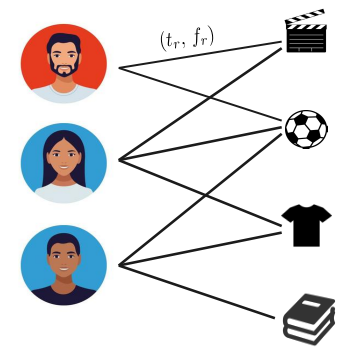
\includegraphics[scale = 0.35]{image/bipartite_graph.png}
    \caption{Bipartite graph}
    \label{bipartite_graph}
\end{figure}
Each interaction is described by a time $t_r$ and a feature vector $f_r$.\\

The claims that the paper made are as follows:
\begin{itemize}
    \item More accurate recommendation performance. By using the JODIE model, the authors claim to obtain better results for the prediction of future interaction on all the datasets used. JODIE outperforms 6 models with an improvement of 20\% in minimum MRR and 14\% in minimum Recall@10.
    \item More accurate state change performance. By using the JODIE model, the authors claim to obtain better results for the change of state of a user on all the data sets used. JODIE outperforms 5 models with an average improvement of 12.63\% in AUC.
    \item Shorter learning time. Thanks to the new t-batch algorithm, learning is 9.2 times faster than other models comparable to JODIE, i.e. with a model with two RNNs.
    \item Robustness of the model to the proportion of the training set. Whatever the percentage of data used for the training data, JODIE outperforms all other models.
    \item The optimal size of the embeddings, found by the authors, is 128.
\end{itemize}

We perform new experiments to demonstrate the impact of the frequency at which the batches are created, i.e the \texttt{split}.
\section*{Methodology}

At first, we wanted to reimplement the code without looking at the authors' original code. We quickly realized that there was a lack of explanation on some technical points like \texttt{t-batch} or neural network inputs. So we decided to use the available code to reimplement the code and improve it. We found that there were details that differed from the paper. The resources we mainly used were the code and the authors' paper. At first, we had a CPU server and then we used a GPU server.\\

The JODIE model is summarised as follows. The model consists of two main components: update operation and projection operation. The update operation is composed of two RNNs that generate user and item embeddings. The projection operator makes a projection in the space of embeddings.

\subsection*{Code}

A publicly available source code has been provided by the original authors in the corresponding \href{https://github.com/srijankr/jodie}{GitHub repository}. It was written using the Pytorch \supercite{NEURIPS2019_bdbca288} library with Python 2.7. A negative point is that the original code was implemented with an outdated version of Python. Another issue was the difficulty encountered in reading the code written in blocks without using functions.\\

Based on the available code, we propose a newer, modular, reusable and understandable version. The use of Python functions facilitates understanding and makes the code modular. Our goal is to reimplement JODIE, in Python 3.8 and Pytorch \supercite{NEURIPS2019_bdbca288} 1.10 a more recent version than the one used in the article.

\subsection*{Model descriptions}

In this section, we will replicate and re-implement the work of Kumar et al. \supercite{kumar2019predicting}. JOint Dynamic user-Item Embedding (JODIE) model is a model that learns dynamic embeddings of users $u_t \in \mathbb{R}^n$, $\forall u \in \mathcal{U}$ and items $i_t \in \mathbb{R}^n$, $\forall i \in \mathcal{I}$ over time t, $\forall t \in [0; T]$, where $\mathcal{U}$ and $\mathcal{I}$ are the sets of users and items and $T$ the final time. Moreover, the interactions are ordered in time, i.e. an interaction between a user $u_r$ and an item $i_r$ at time $t_r$ characterized by $f_r$, noted $S_r = (u_r, \, i_r, \, t_r, \, f_r)$, cannot be before the interaction $S_{r-1}$. The model consists of two main operators: the update operator and the projection operator. To consider the time in the interactions, we cannot separate the data in classical batch, so the authors found a solution called \texttt{t-batch}.

\subsubsection{Architecture and learning}

The architecture consists of two Recurrent Neural Networks (RNNs) and two Multi-Layer Perceptrons (MLP) as shown in Figure \ref{Pipeline}. The first RNN is dedicated to users, the second to items. Both RNNs are activated with sigmoids according to the paper but by looking at the documentation of the RNNCell() function, we saw that the activation function used was hyperbolic tangent. The first MLP is dedicated to user classification. It consists of a hidden layer of 50 neurons activated by a ReLU function and an output layer composed of two neurons, one for each state. The second MLP is dedicated to the estimation of the embedding of the next item. It includes a single projection layer that consists of a linear projection in the space of embeddings.

\begin{figure}[H]
   \begin{center}
        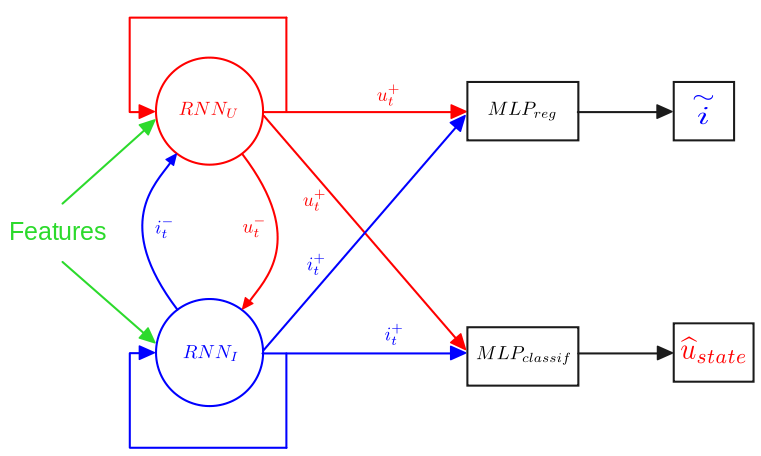
\includegraphics[scale = 0.4]{image/pipeline.png}
    \end{center}
    \caption{Pipeline. $\text{MLP}_{reg}$ gives an estimation of the embedding of the next item $\textcolor{blue}{\overset{\sim}{i}}$ with which a user $\textcolor{red}{u}$ is likely to interact. The MLP  is designed to recommend the best $\textcolor{blue}{i}$ to each user. $\text{MLP}_{classif}$ is used to predict the user's state change $\textcolor{red}{\widehat u_{state}}$. Will the user potentially drop out / get banned ?}
    \label{Pipeline}
\end{figure}

\subsubsection{Update operator}

Now, we will introduce the update operator. The update operator takes the form of two mutually recursive neural networks shown in Figure \ref{recursive RNNs}. The RNN$_u$ is used to update the dynamic user embeddings and the RNN$_i$ updates the dynamic item embeddings. In this case, the embeddings are considered as the hidden state of the classical RNNs respectively. At time $t=0$, we initialize dynamic embeddings $u_0$ and $i_0$ randomly according to a uniform distribution $\mathcal{U}[0;1[$ followed by a normalization which will be used as inputs of the RNNs. As input, there is also the embedding of the other entity, $\Delta$ the time elapsed between an entity and the previous interaction and $f$ a feature vector which characterizes the link of the interaction. A specificity of these RNNs is that they take four inputs instead of two as usual. In order to narrow down to just two entries, we concatenate the embedding of the other entity, $\Delta$ and $f$. In Figure \ref{recursive RNNs}, we denote the concatenation by [.,.]. More formally, we use the following formulas to update the embeddings:
$$
u^+ = \sigma \left ( W_1^u u^- + W_2^u i^- + W_3^u f + W_4^u \Delta_u \right )
$$
$$
i^+ = \sigma \left ( W_1^i i^- + W_2^i u^- + W_3^i f + W_4^i \Delta_i \right )
$$
Where the matrices $W_1^e, ..., W_4^e$ are the parameters of the RNN$_e$ and $\sigma$ an activation function (here hyperbolic tangent). We note by $u^-$ and $i^-$ the embeddings before update and by $u^+$ and $i^+$ the embeddings after update. Once this step is finished, we can proceed to the second operation, the projection operation.

\begin{figure}[H]
   
   \centering
    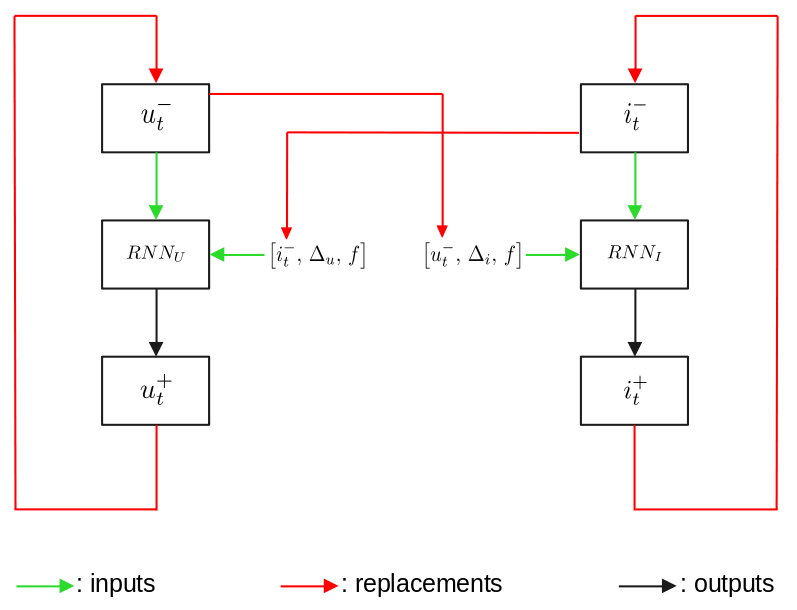
\includegraphics[scale = 0.4]{image/rnn_mutually.png}
    \caption{RNN mutually recursive}
    \label{recursive RNNs}
\end{figure}

\subsubsection{Projection operation}

This operation consists in projecting the user's embedding to a future time. Indeed, it is assumed that user's interest changes with time, for example in winter and in summer, hence the need to model this variation as a linear projection. To make the explanation more clear, the authors present the Figure \ref{Projection} to better understand.\\

\begin{figure}[H]
    \centering
    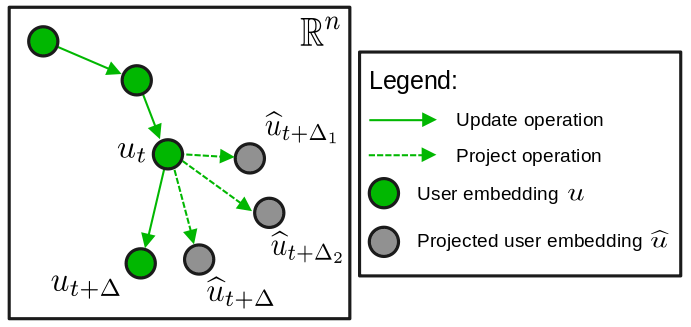
\includegraphics[scale = 0.4]{image/projection_operation.png}
    \caption{Projection operation}
   \label{Projection}
\end{figure}

We notice that over a very short time interval, the projected embedding of the user changes slightly, but as time goes, the projected embedding will be further away from its original embedding. To perform this operation, we must first convert $\Delta$ into a vector $w \in \mathbb{R}^n$ using a linear layer represented by its weights vector $W_p$. We have $w = W_p \Delta$. We initialize $W_p$ by a Gaussian of zero mean. We obtain the projected embedding by computing Hadamard product, denoted $*$, of $1+w$ and $u_t$. The authors use the following formula.
$$
\widehat u_{t+\Delta} = (1+w) * u_t
$$
We can see that if $\Delta = 0$ then $w=0$ and the projected embedding is the same as the initial embedding. We can consider this operation as a simple linear transformation. These two operators consist in the learning of the model. For a faster learning, the authors have created the \texttt{t-batch} algorithm.

\subsubsection{t-Batch algorithm}

The goal of the \texttt{t-batch} algorithm is to be able to separate temporal data in batches. We work on datasets that are indexed by time, so we cannot separate data in a classical batches. Indeed, we cannot update an embedding of a user who arrives at time $t+1$ before an embedding of a user who arrives at time $t$. To do this, we must take into account several constraints. First, the same batch cannot contain the same entity several times. Second, the batches must keep temporal dependencies, i.e. we process the interactions in the order. By respecting these two conditions, the authors guarantee that the batches are parallelizable. A negative point of the original article is the understanding of the \texttt{t-batch} algorithm with only a few lines description. To better understand, we present the algorithm \ref{t-batch}.


%From an algorithmic point of view, those constraint are satisfied while using the algorithm \ref{t-batch}. A negative point of the original article is the understanding of the t-batch algorithm with only a few lines description. To better understand this algorithm, we present it.\\

    \begin{algorithm}[H]
        \caption{t-Batch}
        \label{t-batch}
        \begin{algorithmic} 
            \STATE \textbf{Input} : Sequence of interactions ordered by time $S$ : $S_j = (u_j,\,i_j,\,t_j,\,f_j)$
            \STATE \textbf{Output} : Sequence of batches $B$ : $B_k = \{S_{k,1},\,...,\,S_{k,n} \}$
            \STATE \textbf{Initialize} : 
            \STATE \quad $\text{tbatch\_id\_u[u]} \leftarrow 0 \; \forall \; u \in \mathcal{U}$, \quad $\text{tbatch\_id\_i[i]} \leftarrow 0 \; \forall \; i \in \mathcal{I}$
            \STATE \quad $B_k \leftarrow \{ \},\; \forall \; k \in$ [\![$1,\;\text{Card}(S)$]\!]
            \STATE \quad $C \leftarrow 0$
            \FOR{$S_j \in S$}
                \STATE Extraction $S_j = (u_j,\,i_j,\,t_j,\,f_j)$
                \STATE idx $\leftarrow$ $\max$(tbatch\_id\_u[$u_j$], tbatch\_id\_i[$i_j$]) + 1
                \STATE $B_\text{idx} \leftarrow B_\text{idx} \cup \{ S_j \}$
                \STATE tbatch\_id\_u[$u_j$] = idx
                \STATE tbatch\_id\_i[$i_j$] = idx
                \STATE $C \leftarrow \max(C,\,$idx)
            \ENDFOR
            \RETURN $\{ B_1,\,...,\,B_C \}$
        \end{algorithmic}
    \end{algorithm}


%\begin{algorithm}[H]
%    \caption{t-Batch}
%    \label{t-batch2}
%    \begin{algorithmic} 
%        \STATE \textbf{Input} :  [user\_id, id\_user\_seq, $\Delta_u$, previous\_item\_seq, item\_id, id\_item\_seq, $\Delta_i$,\\
%        \hspace{1.2cm}timestamp\_seq, feature\_seq, y\_true\_labels] = preprocessing(S)\\
%        \hspace{1.1cm} proportion\_train\\
%        \hspace{1.1cm} split
%        \STATE \textbf{Output} : tbatch\_split[${t_1}$] = \{B$_{t_1,1}$, ..., B$_{t_1,n_1}$\} \\
%        \hspace{3.55cm} $\vdots$\\
%        \hspace{1.3cm} tbatch\_split[${t_k}$] = \{B$_{t_k,1}$, ..., B$_{t_k,n_n}$\}\\
%        \hspace{1.3cm} time\_tbatch\_seq = \{$t_1,_,\hdots,\,t_k$\}
%        \STATE \textbf{Initialize} : 
%        \STATE \quad $\text{tbatch\_split}$ $\leftarrow$ \{\}
%        \STATE \quad time\_tbatch\_seq $\leftarrow$ []
%        \STATE \quad $\text{tbatch\_id\_u[u]} \leftarrow 0 \; \forall \; u \in \mathcal{U}$
%        \STATE \quad $\text{tbatch\_id\_i[i]} \leftarrow 0 \; \forall \; i \in \mathcal{I}$
%        \STATE \quad $B_{i,k} \leftarrow \{ \},\; \forall i \in [t_1,\;t_k]\text{ and }\forall \; k \in [1,\;\text{Card}(S)]$
%        \STATE \quad $C \leftarrow 0$
%        \STATE \quad tbatch\_time $\leftarrow$ \textbf{None}
%        \STATE \quad tbatch\_timespan $\leftarrow \frac{\text{timestamp\_seq}_{\text{end}} - \text{timestamp\_seq}_{\text{start}}}{\text{split}}$
%        \FOR{$j \in$ 1 à Card$(S)$}
%            \STATE Extraction $S_j = (u_j,\,i_j,\,t_j,\,f_j)$
%            \STATE idx $\leftarrow$ $\max$(tbatch\_id\_u[$u_j$], tbatch\_id\_i[$i_j$]) + 1
%            \STATE $B_\text{idx} \leftarrow B_\text{idx} \cup \{ S_j \}$
%            \STATE tbatch\_id\_u[$u_j$] = idx
%            \STATE tbatch\_id\_i[$i_j$] = idx
%            \STATE $C \leftarrow \max(C,\,$idx)
%            \IF{tbatch\_time is \textbf{None}}
%            \STATE tbatch\_time $\leftarrow \; t_j$
%            \ENDIF\\
%            \IF{$t_j -$ tbatch\_time > tbatch\_timespan}
%            \STATE tbatch\_split[$t_j$] $\leftarrow$ \{B$_{t_j,1}$, ..., B$_{t_j,C}$\}
%            \STATE time\_tbatch\_seq $\leftarrow$ [$t_j$]
%            \STATE $C \leftarrow 0$
%            \ENDIF
%        \ENDFOR
%        \RETURN tbatch\_split, time\_tbatch\_seq
%    \end{algorithmic}
%\end{algorithm}

The batch index calculation where to place the interaction $r$ is expressed mathematically as:
$$
\text{idx} = \max \left ( \text{maxBatch}(u, \,r-1), \,\text{maxBatch}(i, \,r-1) \right ) + 1
$$
Where $\text{maxBatch}(e, \,r-1)$ gives the index of the biggest batch at time $r-1$ containing the entity $e$ . Thus, we place the interaction in the next batch to respect the temporal dependencies. Moreover, in each batch there is an edge with two nodes of the graph that are totally independent from the other edges in the same batch. By respecting these two conditions, we are guaranteed to make batches that can be parallelized and keep the temporal dependencies. Finally, we do not know the number of batches in advance and the size of the batches will be different. Besides, the \texttt{t-batch} algorithm has a linear complexity. The algorithm goes through each observation only once and is very fast on very large datasets.

\subsubsection{Next item embedding and state change losses}

The JODIE model has been designed to give directly an embedding of an item, which is time saving. Indeed, the existing models predict a probability for each item. This can be very long if the dataset contains many items. JODIE will produce an embedding and the suggested item will be the one whose embedding will be the closest to the one of the prediction. To make this prediction, we use a neural network that will have as input the projected embedding of the user at time $t+\Delta$ noted $\widehat u(t+\Delta)$ and the embedding of the previous item of the user before time $t+\Delta$ noted $i(t+\Delta^-)$. This embedding is important because item can interact with other users between time $t$ and $t+\Delta$, which means that it contains more recent information. JODIE uses both static and dynamic embeddings, denoted respectively $\Bar{e}$ and $e$, to make the prediction of a static and dynamic embedding $\overset{\sim}{i}$. The prediction is done with a fully connected linear layer.
$$
\overset{\sim}{i} (t+\Delta) = W_1 \widehat u(t+\Delta) + W_2 \Bar{u} + W_3 i(t+\Delta^-) + W_4 \Bar{i} + B
$$
Where $W_1, ..., W_4$ and the bias vector $B$ are the model weights.\\

JODIE is trained to minimize the L2 distance between the predicted embedding and the real item embedding of each interaction. We compute the loss function as follows:

\begin{equation}
    \textit{Loss} = \sum_{(u,\,i,\,t,\,f) \in S} \| \overset{\sim}{i}_t - [\Bar{i},\,i_t^-] \|_2 + \lambda_U \|u_t - u_t^-\|_2 + \lambda_I \|i_t - i_t^-\|_2
\end{equation}

The first term minimizes the error of the predicted embedding. The next twos terms regulate the loss function and allow the dynamic embeddings of users and items to not vary too much. $\lambda_U$ and $\lambda_I$ are the regularization terms that penalize the two terms. In the original paper, the authors fixed the values of $\lambda_U$ and $\lambda_I$ as: $\lambda_U = \lambda_I = 1$, without much justification. It is not clear if this is the best value or if another value would be more appropriate. \\

When we want to predict the change of state of a user, we use the same loss function with an additional term which is the cross-entropy. To do this, we have to make sure that the classes are binary. In this case, it is possible to train the model using an additional loss term function that will make it able to predict the labels using the user's embedding after an interaction. The additional loss function term, for predicting a user's state change, is a weighted cross-entropy expressed in the following equation:

\begin{equation}
    \ell(x,y) = \sum_{n=1}^N \frac{l_n}{\sum_{n=1}^N w_{y_n}} \; \text{ with } \;
    l_n = -w_{y_n} \log \left ( \frac{\exp(x_{n,y_n})}{\sum_{c=1}^C \exp(x_{n,c})} \right )
\end{equation}

Where $x$ is the input, $y$ is the target, $w$ is the weight, $C$ is the number of classes (here two) and $N$ is the batch size. The loss function becomes:

\begin{equation}
    \textit{Loss} = \sum_{(u,\,i,\,t,\,f) \in S} \| \overset{\sim}{i}_t - [\Bar{i},\,i_t^-] \|_2 + \lambda_U \|u_t - u_t^-\|_2 + \lambda_I \|i_t - i_t^-\|_2 + \ell (u_{true}, \widehat u_{pred})
\end{equation}

Where $u_{true}$ is the real class of the user and $\widehat u_{pred}$ his predicted class. It is also worth noting that the regularizations terms are MSE. The authors wanted the embeddings not to vary heavily between the previous time $t-1$ and the current time $t$. Indeed, they started from the postulate that the behavior of a user represented by its dynamic embedding does not vary considerably over a small temporal interval.\\

\subsubsection{Training JODIE model} 

We detail the learning steps and the specificity of JODIE model. More precisely, we explain the used functions and we specify there location for a better understanding of the available files.

\begin{enumerate}
    \item We use a function called \textbf{preprocess} which is in the file \textbf{preprocessing.py} to make a pre-processing of the data to extract information necessary during the training. Information like the sequence of users, items, time, features or previous items that will be used in the learning process.
    \item We initialize the embeddings in a unique and same way, i.e. by using a uniform law $\mathcal{U}([0,1[)$.
    \item The JODIE model has a particularity in the way the \texttt{t-batch} is formed, which is not discussed in the article and difficult to understand in the code. Normally to make batches, we cut the dataset with the number of observations we want per batch. But when we have a dataset with temporal dependencies the operation can not be done the same way, this why we apply the \texttt{t-batch} algorithm. But, instead of applying directly the algorithm on the whole dataset, the authors made it in another way. From the temporal data, the authors decided to make subsets of the data and apply independently the \texttt{t-batch} algorithm on each subset of the data. The following figure will help us to understand better:
    \begin{figure}[H]
        \centering
        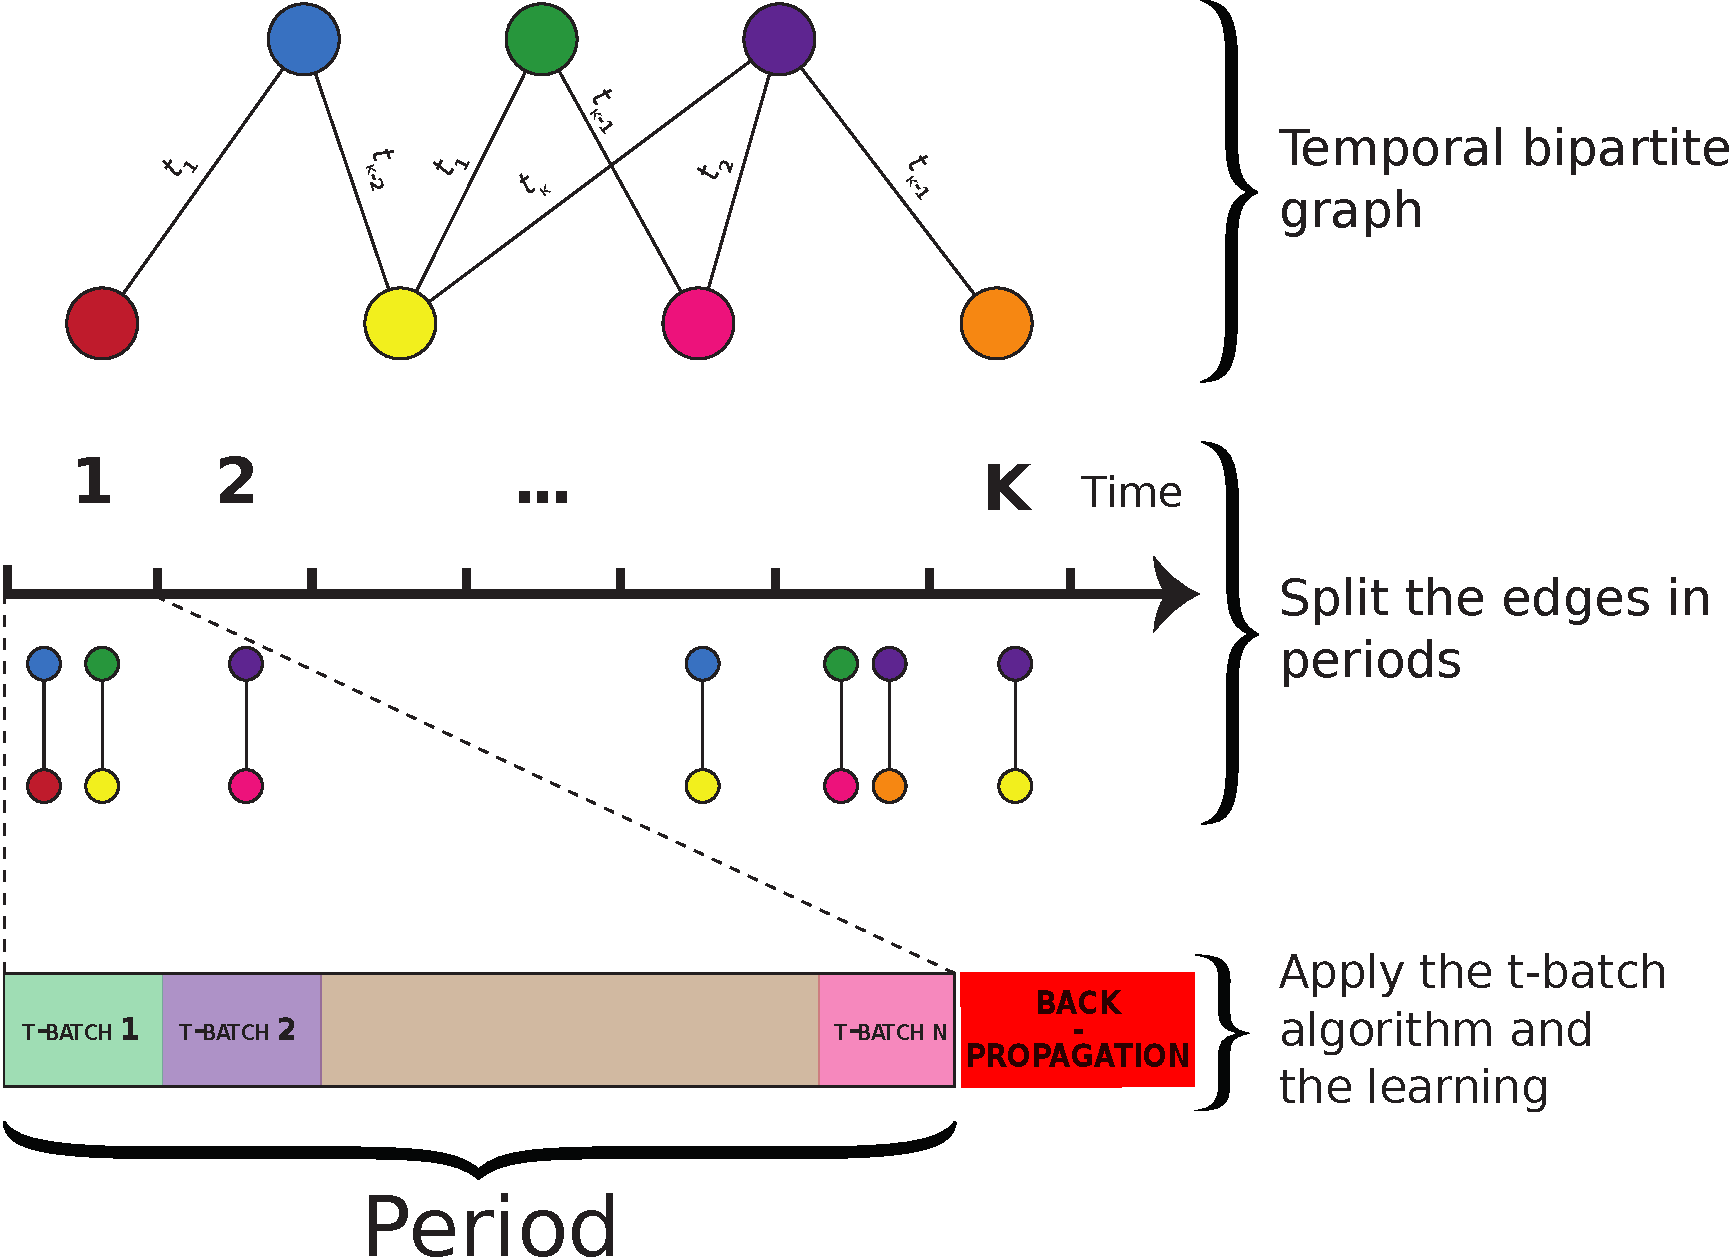
\includegraphics[scale = 0.43]{image/pipeline-jodie.pdf}
        \caption{Pipeline of the \texttt{t-batch} algorithm}
        \label{pipeline_t-batch}
    \end{figure}
    From the temporal bipartite graph, we will separate the edges and classify them in an increasing temporal order. Then, we will take the time interval where the interactions occur and we will divide this time by a hyper-parameter called \texttt{split}. The authors have set \texttt{split} to 500. We obtain temporal periods with different sizes. Finally, we will apply the t-batch algorithm on each period. Once all the t-batches are processed, we can back-propagate the error for one period.
    \item The \texttt{t-batch} algorithm is used to make temporal batches. We use another approach than the authors. Instead of taking a period, applying the \texttt{t-batch} and using the t-batches to learn, we do all the t-batches at once with the function \textbf{t\_batch} in the file \textbf{preprocessing.py} before the learning step and loop over the periods.
    \item During the learning stage, in the function \textbf{train\_ray} in the file \textbf{train.py}, we use the function \textbf{projection} from the file \textbf{model.py} to project the user's embedding in a future time. We also use the function \textbf{predict\_embedding\_item} in the file \textbf{model.py} to make a prediction of the next embedding of the item. And finally, we calculate the Mean Square Error (MSE) of the predicted embedding and the real embedding.
    \item We update the embeddings of users and items using the functions \textbf{update\_rnn\_user} and \textbf{update\_rnn\_item} respectively in the file \textbf{model.py}.
    \item We compute the two regularization terms using the function \textbf{regularizer} of the file \textbf{preprocessing.py}. This function uses the hyperparameter $\lambda_e$.
    \item If necessary, we predict the state prediction and we calculate the loss Cross Entropy (CE) with the function \textbf{loss\_predict\_state} of the file \textbf{model.py} which makes the prediction and the calculation of the loss.
    \item We perform the back-propagation of the gradient, at the end of a period, to update the model weights.
    \item Once all the time periods are covered, we go to the second epoch.
\end{enumerate}
Once the learning stage is over, the evaluation is carried out.

% \begin{comment}
%     \begin{algorithm}[H]
%         \caption{JODIE}
%         \begin{algorithmic} 
%             \STATE \textbf{Input}: Sequence of interactions ordered by time S : $S_j = (u_j,\,i_j,\,t_j,\,f_j)$
%             \STATE \quad \hspace{0.73cm}Initial user embedding $u_t$
%             \STATE \quad \hspace{0.73cm}Initial item embedding $i_t$
%             \STATE \quad \hspace{0.73cm}Current model parameters: $\Theta_{proj}$, $\Theta_{pred}$, $\Theta_{state}$, \textbf{RNN}$_U$, \textbf{RNN}$_I$
%             \STATE \textbf{Output}: Dynamic user and item embeddings, updated model parameters
%             \STATE \textbf{Initialize}: $\ell \leftarrow 0$
%             \STATE \quad \hspace{1.1cm} prev $\leftarrow$ $\{\}$
%             \STATE \quad \hspace{1.1cm} prev$_{state}$ $\leftarrow$ $\{\}$
%             \FOR{$j \in$ 1 à Card$(S)$}
%                 \STATE Preprocessing $S_j$
%                 \STATE $\widehat u_t$ $\; \leftarrow \; \Theta_{proj}(u_t^-, \, \Delta_u)$
%                 \STATE $k \leftarrow$ prev[$u$]
%                 \STATE $\overset{\sim}{i_t} \leftarrow \Theta_{pred}(\widehat u_t, \, \Bar{u}, \, i^-, \,\Bar{i})$
%                 \STATE $\ell \leftarrow \ell + \| \overset{\sim}{i_t} - [ \Bar{i}, \, i_t^-] \|_2$
%                 \STATE $u_t \leftarrow \textbf{RNN}_U(u_t^-,\,i_t^-,\,\Delta_u,\,f)$
%                 \STATE $i_t \leftarrow \textbf{RNN}_I(i_t^-,\,u_t^-,\,\Delta_i,\,f)$
%                 \STATE prev[$u$] $\leftarrow i$
%                 \STATE $\ell \leftarrow \ell + \lambda_u \| u_t - u_t^- \|_2 + \lambda_i \| i_t - i_t^- \|_2$
%                 \IF{State change \TRUE}
%                     \STATE  prev$_{state}[j]$ $\leftarrow$ $u_t$
%                     \STATE $\widehat u_{pred} \leftarrow \Theta_{state}(\text{prev}_{state})$
%                     \STATE $\ell \leftarrow \ell + CE(u_{true},\,\widehat u_{state})$
%                 \ENDIF\\
%                 Back-propagation loss and update model parameters
%             \ENDFOR
%             \RETURN $u_t$, $i_t$, model: $\Theta_{proj}$, $\Theta_{pred}$, $\Theta_{state}$, \textbf{RNN}$_U$, \textbf{RNN}$_I$
%         \end{algorithmic}
%     \end{algorithm}
% \end{comment}


\begin{comment}
\begin{algorithm}[H]
    \caption{JODIE}
    \begin{algorithmic} 
        \STATE \textbf{Input}: Sequence of interactions ordered by time S : $S_j = (u_j,\,i_j,\,t_j,\,f_j)$
        \STATE \quad \hspace{0.73cm}Initial user embedding $u_t$
        \STATE \quad \hspace{0.73cm}Initial item embedding $i_t$
        \STATE \quad \hspace{0.73cm}Current model parameters: $\Theta_{proj}$, $\Theta_{pred}$, $\Theta_{state}$, \textbf{RNN}$_U$, \textbf{RNN}$_I$
        \STATE \quad \hspace{0.73cm}Proportion\_train, split
        \STATE \textbf{Output}: Dynamic user and item embeddings, updated model parameters
        \STATE \textbf{Initialize}: loss\_tbatch $\leftarrow 0$, loss\_total $\leftarrow 0$
        \STATE \quad \hspace{1.2cm} prev $\leftarrow$ $\{\}$, prev$_{state}$ $\leftarrow$ $\{\}$
        \STATE \quad \hspace{1.2cm} [user\_id, id\_user\_seq, $\Delta_u$, previous\_item\_seq, item\_id, id\_item\_seq, $\Delta_i$,\\
        \quad \hspace{1.2cm} timestamp\_seq, feature\_seq, y\_true\_labels] = \textbf{preprocessing}(S)
        \STATE \quad \hspace{1.2cm} [tbatch\_split, time\_tbatch\_seq] = \textbf{tbatch}(user\_id, id\_user\_seq, $\Delta_u$,\\
        \quad \hspace{1.2cm} previous\_item\_seq, item\_id, id\_item\_seq, $\Delta_i$, timestamp\_seq, feature\_seq,\\
        \quad \hspace{1.2cm} y\_true\_labels, proportion\_train, split)
        \FOR{$time$ in time\_tbatch\_seq}
            \FOR{$j$ in tbatch\_split[$time$]}
                \STATE $\widehat u_t$ $\; \leftarrow \; \Theta_{proj}(u_t^-, \, \Delta_u)$
                \STATE $i^- \leftarrow$ prev[$u_t$]
                \STATE $\overset{\sim}{i_t} \leftarrow \Theta_{pred}(\widehat u_t, \, \Bar{u}, \, i^-_t, \,\Bar{i})$
                \STATE loss\_tbatch $\leftarrow$ loss\_tbatch + $\| \overset{\sim}{i_t} - [ \Bar{i}, \, i_t^-] \|_2$
                \STATE $u_t \leftarrow \textbf{RNN}_U(u_t^-,\,i_t^-,\,\Delta_u,\,f)$
                \STATE $i_t \leftarrow \textbf{RNN}_I(i_t^-,\,u_t^-,\,\Delta_i,\,f)$
                \STATE prev[$u_t$] $\leftarrow i$
                \STATE loss\_tbatch $\leftarrow$ loss\_tbatch + $\lambda_u \| u_t - u_t^- \|_2 + \lambda_i \| i_t - i_t^- \|_2$
                \IF{State \textbf{True}}
                    \STATE  prev$_{state}[j]$ $\leftarrow$ $u_t$
                    \STATE $\widehat u_{pred} \leftarrow \Theta_{state}(\text{prev}_{state})$
                    \STATE loss\_tbatch $\leftarrow$ loss\_tbatch + $CE(u_{true},\,\widehat u_{pred})$
                \ENDIF\\
            \ENDFOR\\
            loss\_total $\leftarrow$ loss\_total + loss\_tbatch\\
            loss\_tbatch $\leftarrow$ 0\\
            Back-propagation loss and update model parameters
        \ENDFOR
        \RETURN $u_t$, $i_t$, model: $\Theta_{proj}$, $\Theta_{pred}$, $\Theta_{state}$, \textbf{RNN}$_U$, \textbf{RNN}$_I$
    \end{algorithmic}
\end{algorithm}
\end{comment}

\subsubsection{Evaluate JODIE model}

The prediction and evaluation stage are just as special as the learning stage. In the evaluation, there is still a "learning" because during the predictions, the model will update itself respecting the time of the periods defined by \texttt{split}. This evaluation is done thanks to the function \textbf{evaluate} of the file \textbf{evaluate.py}. During the evaluation, we do not apply the \texttt{t-batch} algorithm on the remaining interactions, but we will treat them one after the other (figure \ref{pipeline_t-batch} not t-batch but interaction just before the back-propagation).


From a temporal bipartite graph, we proceed in the same way as for learning, we separate the edges in temporal order. Then, we will separate the data into periods and we will process the interactions one after the other. The periods are defined with the hyper-parameter \texttt{split} as for the periods of the \texttt{t-batch}. In addition to all the learning steps in the evaluation, we add a prediction step. According to the prediction task, we will predict a probability of a user's state change using the function \textbf{predict\_state} in the file \textbf{model.py}. Otherwise we will predict an embedding and look for the item which has its closest embedding in terms of Euclidean distance. Finally, we will calculate the metrics to obtain the validation and generalization error.

\begin{comment}
\begin{algorithm}[H]
    \caption{Evaluation of future interaction prediction}
    \begin{algorithmic} 
        \STATE \textbf{Input}: hyperparameters: embedding\_size, split, $\lambda_u$, $\lambda_i$
        \STATE \quad \hspace{0.73cm}Sequence of interactions ordered by time S : $S_j = (u_j,\,i_j,\,t_j,\,f_j)$
        \STATE \quad \hspace{0.73cm}State $\leftarrow$ False 
        \STATE \quad \hspace{0.73cm}Proportion\_train
        \STATE \textbf{Output}: perf\_val, perf\_test
        \STATE \textbf{Initialize}: [user\_id, id\_user\_seq, $\Delta_u$, previous\_item\_seq, item\_id, id\_item\_seq, $\Delta_i$,\\
        \quad \hspace{1.2cm} timestamp\_seq, feature\_seq, y\_true\_labels] = \textbf{preprocessing}(S)
        \STATE \quad \hspace{1.2cm} $u_t$, $i_t$, $\Theta_{proj}$, $\Theta_{pred}$, $\Theta_{state}$, \textbf{RNN}$_U$, \textbf{RNN}$_I$ = \textbf{load\_model}(hyperparameters)
        \STATE \quad \hspace{1.2cm} tbatch\_timespan $\leftarrow \frac{\text{timestamp\_seq}_{\text{end}} - \text{timestamp\_seq}_{\text{start}}}{\text{split}}$
        \STATE \quad \hspace{1.2cm} idx\_train = Card(S) * (proportion\_train)
        \STATE \quad \hspace{1.2cm} idx\_val = Card(S) * (proportion\_train + ($\frac{1 - \text{proportion\_train}}{2}$))
        \STATE \quad \hspace{1.2cm} idx\_test = Card(S)
        \STATE \quad \hspace{1.2cm} tbatch\_time $\leftarrow$ \textbf{None}
        \STATE \quad \hspace{1.2cm} loss $\leftarrow$ 0
        \STATE \quad \hspace{1.2cm} val\_rank $\leftarrow$ [], test\_rank $\leftarrow$ []
        \FOR{$j$ in (idx\_train : idx\_test)}
            \STATE Extraction $S_j = (u_j,\,i_j,\,t_j,\,f_j)$
            \IF{tbatch\_time is \textbf{None}}
                \STATE tbatch\_time $\leftarrow$ $t_j$
            \ENDIF
            \STATE $\widehat u_j$ $\; \leftarrow \; \Theta_{proj}(u_j^-, \, \Delta_u)$
            %\STATE $i^- \leftarrow$ prev[$u_j$]
            \STATE $\overset{\sim}{i_j} \leftarrow \Theta_{pred}(\widehat u_j, \, \Bar{u}, \, i^-_j, \,\Bar{i})$
            \STATE loss $\leftarrow$ loss + $\| \overset{\sim}{i_j} - [ \Bar{i}, \, i_j^-] \|_2$
            \STATE euclidean\_dist $\leftarrow$ \textbf{Dist}($\overset{\sim}{i_j}$, all\_embeddings\_items)
            \STATE euclidean\_dist\_smaller $\leftarrow$ (euclidean\_dist < euclidean\_dist[$i_j$])
            \STATE true\_item\_rank $\leftarrow$ \textbf{sum}(euclidean\_dist\_smaller) + 1
            \IF{$j$ < idx\_val}
                \STATE val\_rank $\leftarrow$ [true\_item\_rank]
            \ELSE
                \STATE test\_rank $\leftarrow$ [true\_item\_rank]
            \ENDIF
            \STATE $u_j \leftarrow \textbf{RNN}_U(u_j^-,\,i_j^-,\,\Delta_u,\,f_j)$
            \STATE $i_j \leftarrow \textbf{RNN}_I(i_j^-,\,u_j^-,\,\Delta_i,\,f_j)$
            %\STATE prev[$u_t$] $\leftarrow i$
            \STATE loss $\leftarrow$ loss + $\lambda_u \| u_j - u_j^- \|_2 + \lambda_i \| i_j - i_j^- \|_2$
            \IF{$t_j - \text{tbatch\_time}$ > tbatch\_timespan}
                \STATE tbatch\_time $\leftarrow$ $t_j$
                \STATE Back-propagation loss and update model parameters
                \STATE loss $\leftarrow$ 0
            \ENDIF
        \ENDFOR\\
        \STATE mrr\_val = \textbf{mean}($\frac{1}{r}$, for $r$ in val\_rank)
        \STATE recall10\_val = $\frac{\textbf{sum}(\text{val\_rank} \leq 10)}{\text{len(val\_rank)}}$
        \STATE mrr\_test = \textbf{mean}($\frac{1}{r}$, for $r$ in test\_rank)
        \STATE recall10\_test = $\frac{\textbf{sum}(\text{test\_rank} \leq 10)}{\text{len(test\_rank)}}$
        \STATE perf\_val $\leftarrow$ [mrr\_val, recall10\_val]
        \STATE perf\_test $\leftarrow$ [mrr\_test, recall10\_test]
        \RETURN perf\_val, perf\_test
    \end{algorithmic}
\end{algorithm}
\end{comment}

\begin{comment}
\begin{algorithm}[H]
    \caption{Evaluation of user state change prediction}
    \begin{algorithmic} 
        \STATE \textbf{Input}: hyperparameters: embedding\_size, split, $\lambda_u$, $\lambda_i$
        \STATE \quad \hspace{0.73cm}Sequence of interactions ordered by time S : $S_j = (u_j,\,i_j,\,t_j,\,f_j)$
        \STATE \quad \hspace{0.73cm}State $\leftarrow$ True
        \STATE \quad \hspace{0.73cm}Proportion\_train
        \STATE \textbf{Output}: perf\_val, perf\_test
        \STATE \textbf{Initialize}: [user\_id, id\_user\_seq, $\Delta_u$, previous\_item\_seq, item\_id, id\_item\_seq, $\Delta_i$,\\
        \quad \hspace{1.2cm} timestamp\_seq, feature\_seq, y\_true\_labels] = \textbf{preprocessing}(S)
        \STATE \quad \hspace{1.2cm} $u_t$, $i_t$, $\Theta_{proj}$, $\Theta_{pred}$, $\Theta_{state}$, \textbf{RNN}$_U$, \textbf{RNN}$_I$ = \textbf{load\_model}(hyperparameters)
        \STATE \quad \hspace{1.2cm} tbatch\_timespan $\leftarrow \frac{\text{timestamp\_seq}_{\text{end}} - \text{timestamp\_seq}_{\text{start}}}{\text{split}}$
        \STATE \quad \hspace{1.2cm} idx\_val = Card(S) * (proportion\_train)
        \STATE \quad \hspace{1.2cm} idx\_val = Card(S) * (proportion\_train + ($\frac{1 - \text{proportion\_train}}{2}$))
        \STATE \quad \hspace{1.2cm} idx\_test = Card(S)
        \STATE \quad \hspace{1.2cm} tbatch\_time $\leftarrow$ \textbf{None}
        \STATE \quad \hspace{1.2cm} loss $\leftarrow$ 0
        \STATE \quad \hspace{1.2cm} val\_pred $\leftarrow$ [], val\_true $\leftarrow$ [], test\_pred $\leftarrow$ [], test\_true $\leftarrow$ []
        \FOR{$j$ in (idx\_train : idx\_test)}
            \STATE Extraction $S_j = (u_j,\,i_j,\,t_j,\,f_j)$
            \IF{tbatch\_time is \textbf{None}}
                \STATE tbatch\_time $\leftarrow$ $t_j$
            \ENDIF
            \STATE $\widehat u_j$ $\; \leftarrow \; \Theta_{proj}(u_j^-, \, \Delta_u)$
            \STATE $\overset{\sim}{i_j} \leftarrow \Theta_{pred}(\widehat u_j, \, \Bar{u}, \, i^-_j, \,\Bar{i})$
            \STATE loss $\leftarrow$ loss + $\| \overset{\sim}{i_j} - [ \Bar{i}, \, i_j^-] \|_2$
            \STATE $u_j \leftarrow \textbf{RNN}_U(u_j^-,\,i_j^-,\,\Delta_u,\,f_j)$
            \STATE $i_j \leftarrow \textbf{RNN}_I(i_j^-,\,u_j^-,\,\Delta_i,\,f_j)$
            \STATE loss $\leftarrow$ loss + $\lambda_u \| u_j - u_j^- \|_2 + \lambda_i \| i_j - i_j^- \|_2$
            \STATE  prev$_{state}[j]$ $\leftarrow$ $u_j$
            \STATE $\widehat u_{pred} \leftarrow \Theta_{state}(\text{prev}_{state})$
            \STATE loss $\leftarrow$ loss + $CE(u_{true},\,\widehat u_{pred})$
            \IF{$t_j - \text{tbatch\_time}$ > tbatch\_timespan}
                \STATE tbatch\_time $\leftarrow$ $t_j$
                \STATE Back-propagation loss and update model parameters
                \STATE loss $\leftarrow$ 0
            \ENDIF
            \STATE proba $\leftarrow$ \textbf{MLP}($u_j$)
            \IF{$j$ < idx\_val}
                \STATE val\_pred $\leftarrow$ [proba]
                \STATE val\_true $\leftarrow$ [y\_true\_labels[$j$]]
            \ELSE
                \STATE test\_pred $\leftarrow$ [proba]
                \STATE test\_true $\leftarrow$ [y\_true\_labels[$j$]]
            \ENDIF
        \ENDFOR\\
        \STATE perf\_val $\leftarrow$ [AUC(val\_true, val\_pred)]
        \STATE perf\_test $\leftarrow$ [AUC(test\_true, test\_pred)]
        \RETURN perf\_val, perf\_test
    \end{algorithmic}
\end{algorithm}
\end{comment}

\subsection*{Datasets}
 % dire que les données sont données par les auteurs mais qu'elles ont un format bizarre et qu'il a fallu traiter les données.
 
The data sets that were used in the original article were also used in this work. The authors of the article give the datasets. \\

\textbf{Reddit\supercite{Reddit} post dataset}: this public dataset consists of one month of posts made by users on subreddits. We selected the 1000 most active subreddits as items and the 10000 most active users. We convert the text of each post into a feature vector representing their Linguistic Inquiry and Work Count\supercite{pennebaker01LIWC} (LIWC) categories.\\
\textbf{Wikipedia\supercite{Wiki} edits}: this public dataset is one month of edits made by edits on Wikipedia pages. We selected the 1000 most edited pages as items and editors who made at least 5 edits as users (a total of 8227 users). Similar to the Reddit dataset, we convert the edit text into a LIWC feature vector.\\
\textbf{LastFM\supercite{10.1007/978-3-642-33486-3_5lastFM} song listens}: this public dataset has one month of who-listens-to-which song information. We selected all 1000 users and the 1000 most listened songs. In the dataset, interactions do not have features.\\
\textbf{Reddit bans}: Reddit post dataset with ground-truth labels of banned users from Reddit. This gives 366 true labels (=0.05\%).\\
\textbf{Wikipedia bans}: Wikipedia edit data with public ground-truth labels of banned users. This results in 217 positive labels (=0.14\%).\\
\textbf{MOOC\supercite{mooc} student drop-out}: this public dataset consists of actions done by students on a MOOC online course. This dataset consists of 7047 users interacting with 98 items. There are 4066 drop-out events (=0.98\%). All datasets and their details are shown in table \ref{description data}. \\

\begin{table}[H]
    \centering
    \ra{1.3}
    \begin{tabular}{@{}lrrrrcc@{}}
    \toprule
    & Users & Items & Interactions & State changes & Action repetition & Features size \\
    \midrule
    Reddit & 10,000 & 984 & 672,447 & 366 & 79\% & 172 \\
    Wikipedia & 8,227 & 1,000 & 157,474 & 217 & 61\% & 172 \\
    LastFM & 980 & 1,000 & 1,293,103 & -\textcolor{white}{0} & 8.6\% & 2 \\
    MOOC & 7,047 & 97 & 411,749 & 4,066 & - & 4 \\
    \bottomrule
    \end{tabular}
    \caption{Description of the datasets that were used in this project}
    \label{description data}
\end{table}

The authors of the original paper created their own datasets. Thus, a dataset has the following format :
\begin{itemize}
    \item A line represents an interaction or an edge
    \item Each line is described by a user, an item, a timestamp, a state label and features
    \item The timestamp is in cardinal number format
    \item The state label is 1 if the user changes state and 0 otherwise. If there are no state labels, use 0 for all interactions
    \item Features can be as long as desired and of dimension at least 1. If there is no feature, use 0 for all interaction
\end{itemize}
A negative point about the data sets is that the variable names are not in the right places and this creates errors when using them. That is why we created a function called \textbf{fetch\_datasets} in the file \textbf{preprocessing.py} which allows to have correct variable names which have the following format: \texttt{user, item, timestamp, labels, f\_1, ..., f\_$n$} with $n$ the number of features.\\

\subsection*{Hyperparameters}

As described in the model descriptions section, the model has several hyperparameters like epoch number, dynamic embedding size, learning rate, \texttt{split}, $\lambda_U$ and $\lambda_I$. Initially the hyperparameters were chosen as in the original article as follow.

\begin{itemize}
    \item Embedding size: $32, \, 64, \, \boldsymbol{128}, \, 256$
    \item Epoch, learning rate, $\lambda_U$ and $\lambda_I$: $50, \, 1e-3, \, 1, \, 1$ respectively
    \item \texttt{Split}: $500$
\end{itemize}

\begin{comment}
\begin{table}[H]
    \centering
    \begin{tabular}{|c|c|c|c|c|}
        \cline{2-5} \multicolumn{1}{c|}{} & \multicolumn{4}{c|}{JODIE}\\
        \cline{2-5} \multicolumn{1}{c|}{} & Reddit & Wikipedia & LastFM & MOOC \\\hline
        Epochs & 50 & 50 & 50 & 50 \\\hline
        Dynamic embedding size & 128 & 128 & 128 & 128 \\\hline
        Learning rate & 0.001 & 0.001 & 0.001 & 0.001 \\\hline
        Split & 500 & 500 & 500 & 500 \\\hline
        $\lambda_U$ & 1 & 1 & 1 & 1 \\\hline
        $\lambda_I$ & 1 & 1 & 1 & 1 \\\hline
    \end{tabular}
    \caption{Hyperparameters details on all datasets}
\end{table}
\end{comment}
Only the size of the dynamic embeddings have been studied and chosen using a grid search. The other hyperparameters are just given without any justification.

\subsection*{Extended experiments}

Of all these hyper-parameters, the one that caught our eye the most was \texttt{split}. Indeed, \texttt{split} is used to define the frequency at which t-batches are created and the JODIE model is trained. It is important to choose its value well to have enough data in a period. To test this hyper-parameter, we set the other hyper-parameters to $50$ epoch, $\lambda_U = \lambda_I = 1$, learning rate = $1e-3$ and the size of the embeddings to $128$, and we test these $5$, $500$ and $50000$ for the value of \texttt{split}. We define \texttt{split} as follows:
\texttt{split} is used to split the dataset for a specific period of time. The authors use it as follows : $\frac{\text{time}_{\text{end}} - \text{time}_{\text{start}}}{\text{\texttt{split}}}$

\section*{Results}

In this section, we will present the results obtained with replication. First, we tried to replicate the results for the user's state change prediction on all available datasets. The strategy  was to predict only with the model weights obtained in the last learning epoch while the authors decided to keep the best epochs weights. For this prediction task, other embedding sizes were tested like 8, 16 and 32. Then, we tried to reproduce the results for the future interaction prediction using the same strategy as for the state prediction. Then a second part was devoted to adding results that are not present in the original paper like the importance of the \texttt{split} hyper-parameter.

\subsection*{Core replication results}
The first part of the results concerns the prediction of the user's state change. The model has for hyperparameters a \texttt{split} of $500$, $\lambda_U = \lambda_I = 1$ as those in the original paper and the embedding size varies. We present the results obtained for embeddings of size $32$, $128$ and $256$ as well as the results of the original paper in the following table:
%\begin{table}[H]
%    \centering
%    \ra{1.3}
%    \begin{tabular}{@{}cccc@{}}\toprule
%            Method & Reddit & Wikipedia & MOOC \\\hline
%        JODIE (embedding size: 128) & \textbf{0.599} & \textbf{0.831} & \textbf{0.756}\\\hline
%        JODIE replication (embedding size: 32) & 0.576 & 0.731 & 0.565 \\\hline
%        JODIE replication (embedding size: 128) & 0.576 & 0.778 & 0.721 \\\hline
%        JODIE replication (embedding size: 256) & 0.551 & 0.747 & 0.705 \\\hline
%    \end{tabular}
%    \caption{Results: user state change prediction}
%\end{table}

\begin{table}[H]
    \centering
    \ra{1.3}
    \begin{tabular}{@{}lcrrrr@{}}
    \toprule
    & JODIE & \phantom{abc} & \multicolumn{3}{c}{Replications} \\
    \cmidrule{2-2} \cmidrule{4-6}
    & 128 && \multicolumn{1}{c}{32} & \multicolumn{1}{c}{128} & \multicolumn{1}{c}{256} \\
    \midrule
    Reddit & $\boldsymbol{0.599}$ && $0.563 \pm 0.013$ & $0.586 \pm 0.018$ & $0.577 \pm 0.012$\\
    Wikipedia &$\boldsymbol{0.831}$ && $0.728 \pm 0.010$ & $0.738 \pm 0.030$ & $0.711 \pm 0.008$\\
    MOOC &$\boldsymbol{0.756}$ && $0.688 \pm 0.006$ & $0.718 \pm 0.021$ & $0.711 \pm 0.004$\\
    \bottomrule
    \end{tabular}
    \caption{Results: user state change prediction}
\end{table}

We observe for the Reddit dataset, a performance of $0.586$ AUC for the reproduction against $0.599$ in the original paper. We also notice a  $0.718$ AUC  for the MOOC dataset results which is close to the $0.756$ AUC obtained in the original paper. For Wikipedia dataset, we can observe a performance of $0.738$ AUC for the reproduction and $0.831$ AUC for the original model. On the Reddit, Wikipedia and MOOC datasets, we see a standard deviation of $0.018$, $0.030$ and $0.021$ respectively for an embedding size of 128. We can explain this difference by the fact that the authors of JODIE evaluated their models on each epoch and chose the best performance in validation while our results come from the 50 and last epoch. This can explain the difference between their results and our results but this difference remains nevertheless minimal.\\
We can see that if we increase the size of the embeddings to 256, the results degrade slightly. This can be due to size of the embeddings which is too big which allows fitting some noise from the data. Conversely, if the size of the embeddings is 32, the results are worse. This can be explained by the fact that the embeddings are too small and lack information to make a good prediction.\\

For the prediction of future interaction, we used the same hyperparameters as for the state prediction. We present the obtained results and the results of the original paper in the following table:

%\begin{table}[H]
%    \hspace{-2.3cm}
%    \begin{tabular}{|c|c|c|c|c|c|c|}
%        \cline{2-7} \multicolumn{1}{c|}{} & \multicolumn{2}{c|}{Reddit} & \multicolumn{2}{c|}{Wikipedia} & \multicolumn{2}{c|}{LastFM}\\
%        \cline{1-7} \multicolumn{1}{|c|}{Method} & MRR & Recall@10 & MRR & Recall@10 & MRR & Recall@10 \\\hline
%        JODIE (embedding size: 128) & \textbf{0.726} & \textbf{0.852} & \textbf{0.746} & \textbf{0.822} & \textbf{0.195} & \textbf{0.307} \\\hline
%        JODIE replication (embedding size: 128) & 0.707 & 0.799 & 0.765 & 0.835 & 0.312 & 0.551 \\\hline
%        JODIE replication (embedding size: 256) & 0.688 & 0.756 & 0.755 & 0.812 & 0.313 & 0.455 \\\hline
%    \end{tabular}
%    \caption{Results: future interaction prediction}
%\end{table}

\begin{table}[H]
    \centering
    \ra{1.3}
    \begin{tabular}{@{}lccccc@{}}
    \toprule
    Dataset\hspace*{3em} & JODIE & \phantom{abc} & \multicolumn{3}{c}{Replications} \\
    \cmidrule{2-2} \cmidrule{4-6}
    & 128 && \multicolumn{1}{c}{32} & \multicolumn{1}{c}{128} & \multicolumn{1}{c}{256} \\
    \midrule
    \multicolumn{1}{l}{\hspace{-0.2cm}\textbf{Reddit}} \\
    {\quad \small MRR} & $\boldsymbol{0.726}$  && $0.711 \pm 0.007$ & $0.719 \pm 0.008$ & $0.684 \pm 0.005$ \\
    {\quad\small Recall@10}  &$\boldsymbol{0.852}$ && $0.810 \pm 0.020$ & $0.830 \pm 0.020$ & $0.747 \pm 0.011$\\
    \multicolumn{1}{l}{\hspace{-0.2cm}\textbf{Wikipedia}}\\
    {\quad\small MRR} &$\boldsymbol{0.746}$ && $0.763 \pm 0.005$ & $0.764 \pm 0.002$ & $0.763 \pm 0.004$  \\
    {\quad\small Recall@10}  & $\boldsymbol{0.822}$ && $0.829 \pm 0.005$ & $0.833 \pm 0.004$ & $0.827 \pm 0.004$\\
    \multicolumn{1}{l}{\hspace{-0.2cm}\textbf{LastFM}} \\
    {\quad\small MRR} &$\boldsymbol{0.195}$ && $0.311 \pm 0.001$ & $0.313 \pm 0.002$ & $0.312 \pm 0.001$ \\
    {\quad\small Recall@10}  & $\boldsymbol{0.307}$ && $0.455 \pm 0.003$ & $0.483 \pm 0.047$ & $0.453 \pm 0.002$\\
    \bottomrule
    \end{tabular}
    \caption{Results: future interaction prediction}
\end{table}

We notice that only the results for the Reddit dataset are slightly lower than in the original paper. On these data, we obtained 0.719 in MRR and 0.830 in Recall@10. However, these results remain close to those obtained by the authors with 0.726 in MRR and 0.852 in Recall@10. For the Wikipedia and LastFM datasets, we can see that our results outperformed the authors' results with 0.764 in MRR and 0.833 in Recall@10 and 0.313 in MRR and 0.483 in Recall@10 respectively. These differences can be explained by the choice to evaluate the last epoch and not to choose the best performance on the validation. These differences remain small. we can also see that the standard deviations, of the different data sets, are low.\\

To go further in the replication and reproduction, we will also reproduce two figures that show that the robustness of JODIE model. The first figure will concern the prediction of future interaction on the Wikipedia dataset by plotting the MRR. For this figure, we varied the percentage of the training set from 10\% to 80\% with 10\% step. The second figure will be on the same dataset but for the prediction of user state change. For this, we varied the percentage of the training set from 20\% to 60\% in 10\% steps.

% \begin{figure}[H]
% 	\centering
%     \subfigure[A]{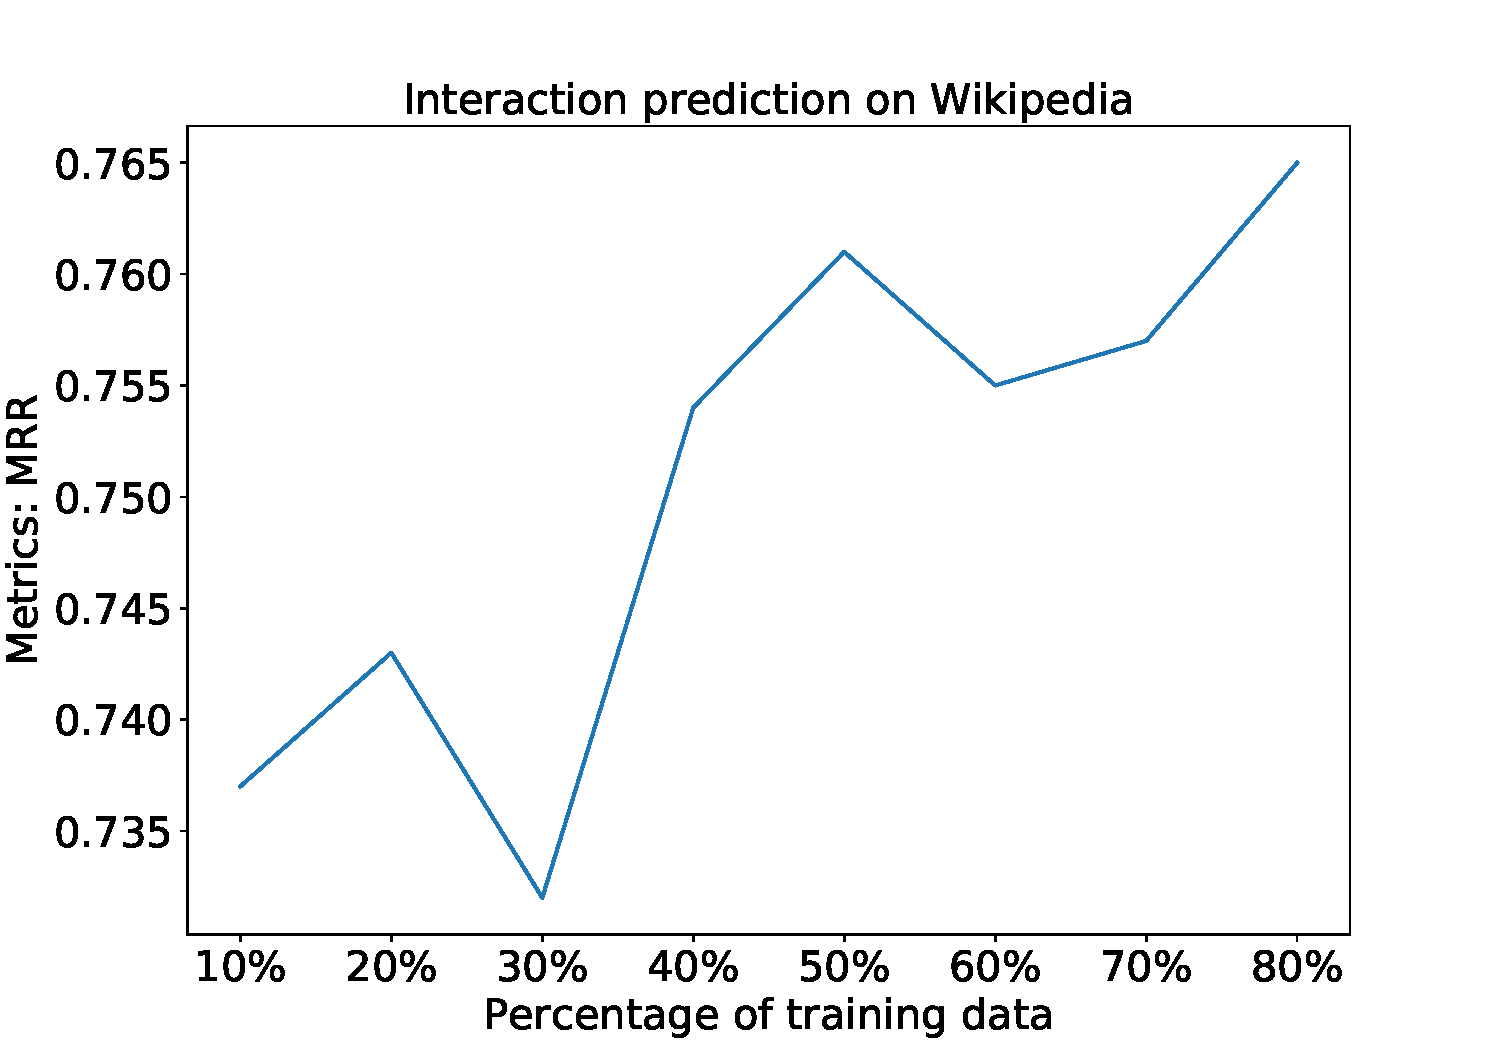
\includegraphics[width=0.46\textwidth]{image/wiki.pdf}} 
%     \subfigure[B]{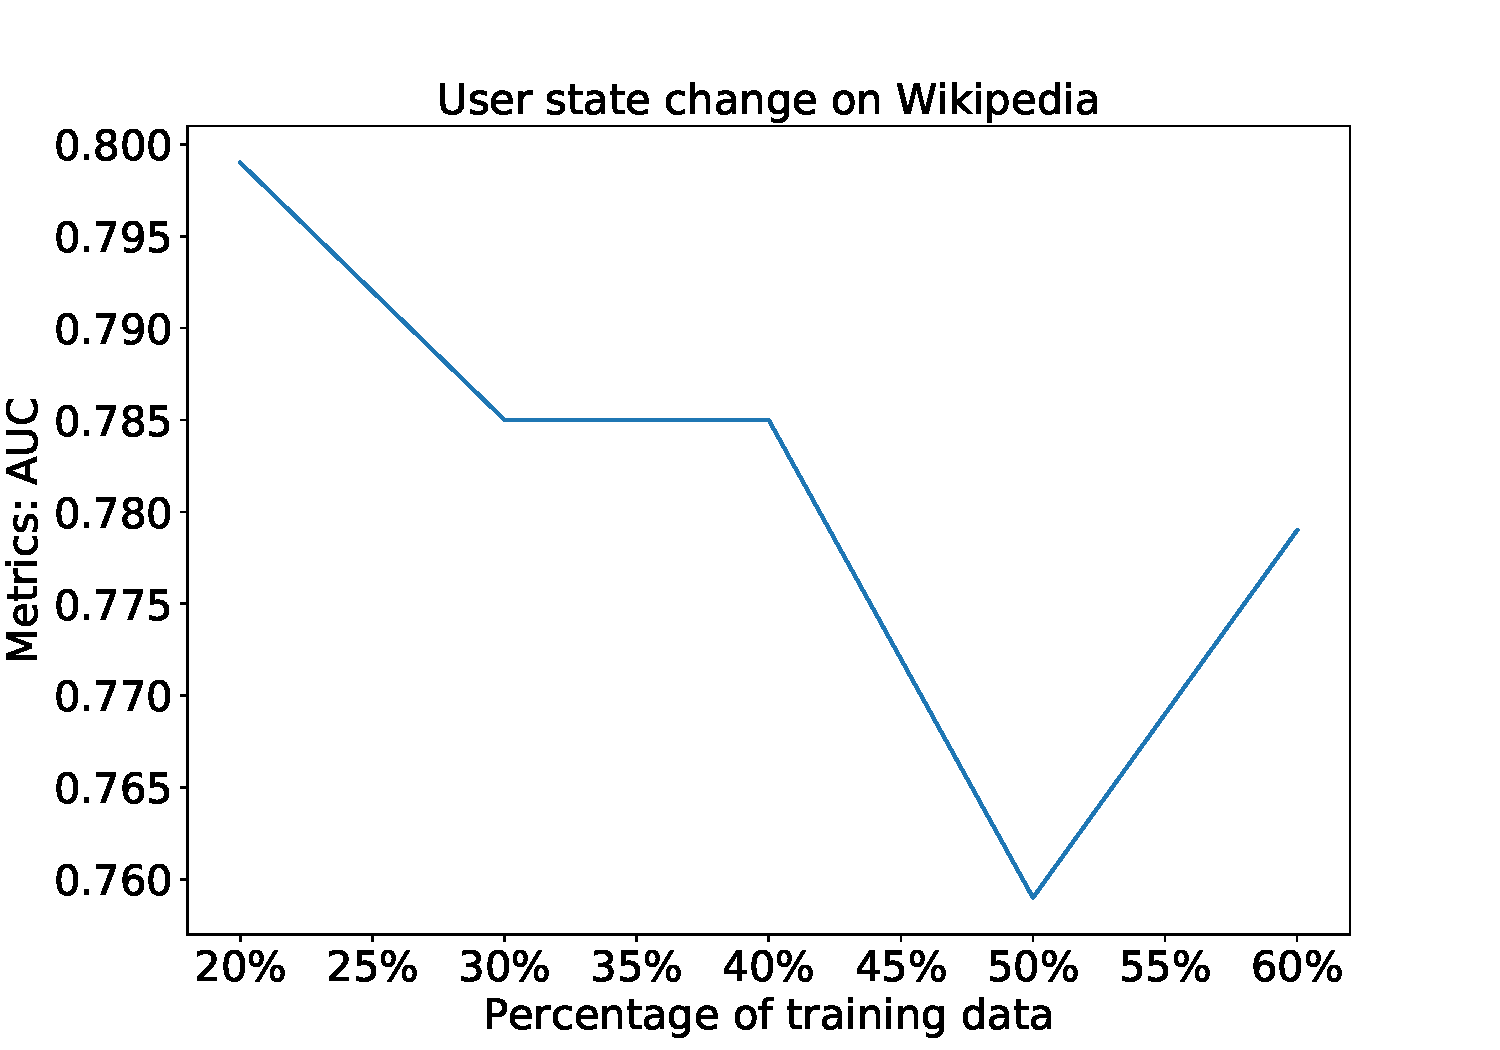
\includegraphics[clip,width=0.46\textwidth]{image/wiki_state.pdf}}
%     \caption{Robustness of JODIE replication: [A] compare the MRR of JODIE replication with baselines on interaction prediction task, by varying the training data size. [B] shows the AUC of user state change prediction task by varying the training data size.}
%     \label{fig:foobar}
% \end{figure}


\begin{figure}[H]
    \centering
    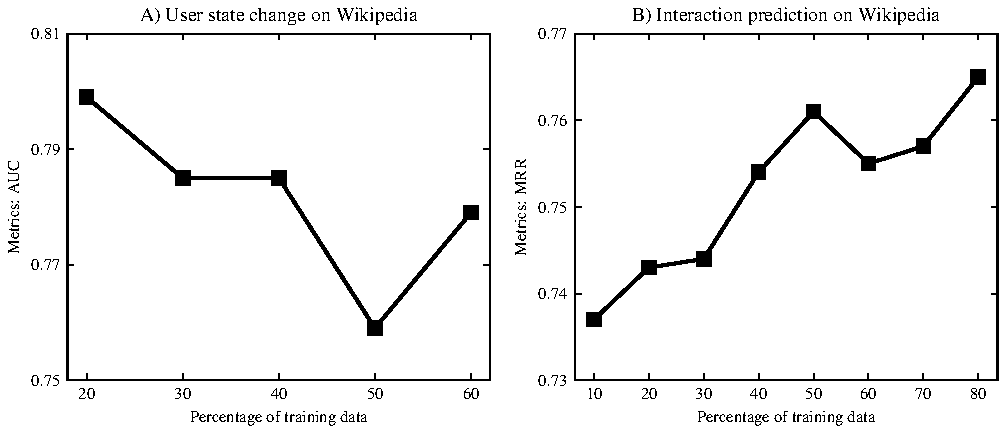
\includegraphics[width = \textwidth]{image/percentage_train.pdf}
    \caption{Robustness of JODIE replication: the figure on the right compare the MRR of JODIE replication with baselines on interaction prediction task, by varying the training data size. The figure on the left shows the AUC of user state change prediction task by varying the training data size.}
    \label{fig:my_label}
\end{figure}


%\begin{figure}[H]
%	\centering
%    \begin{subfigure}[b]{0.49\textwidth}
%        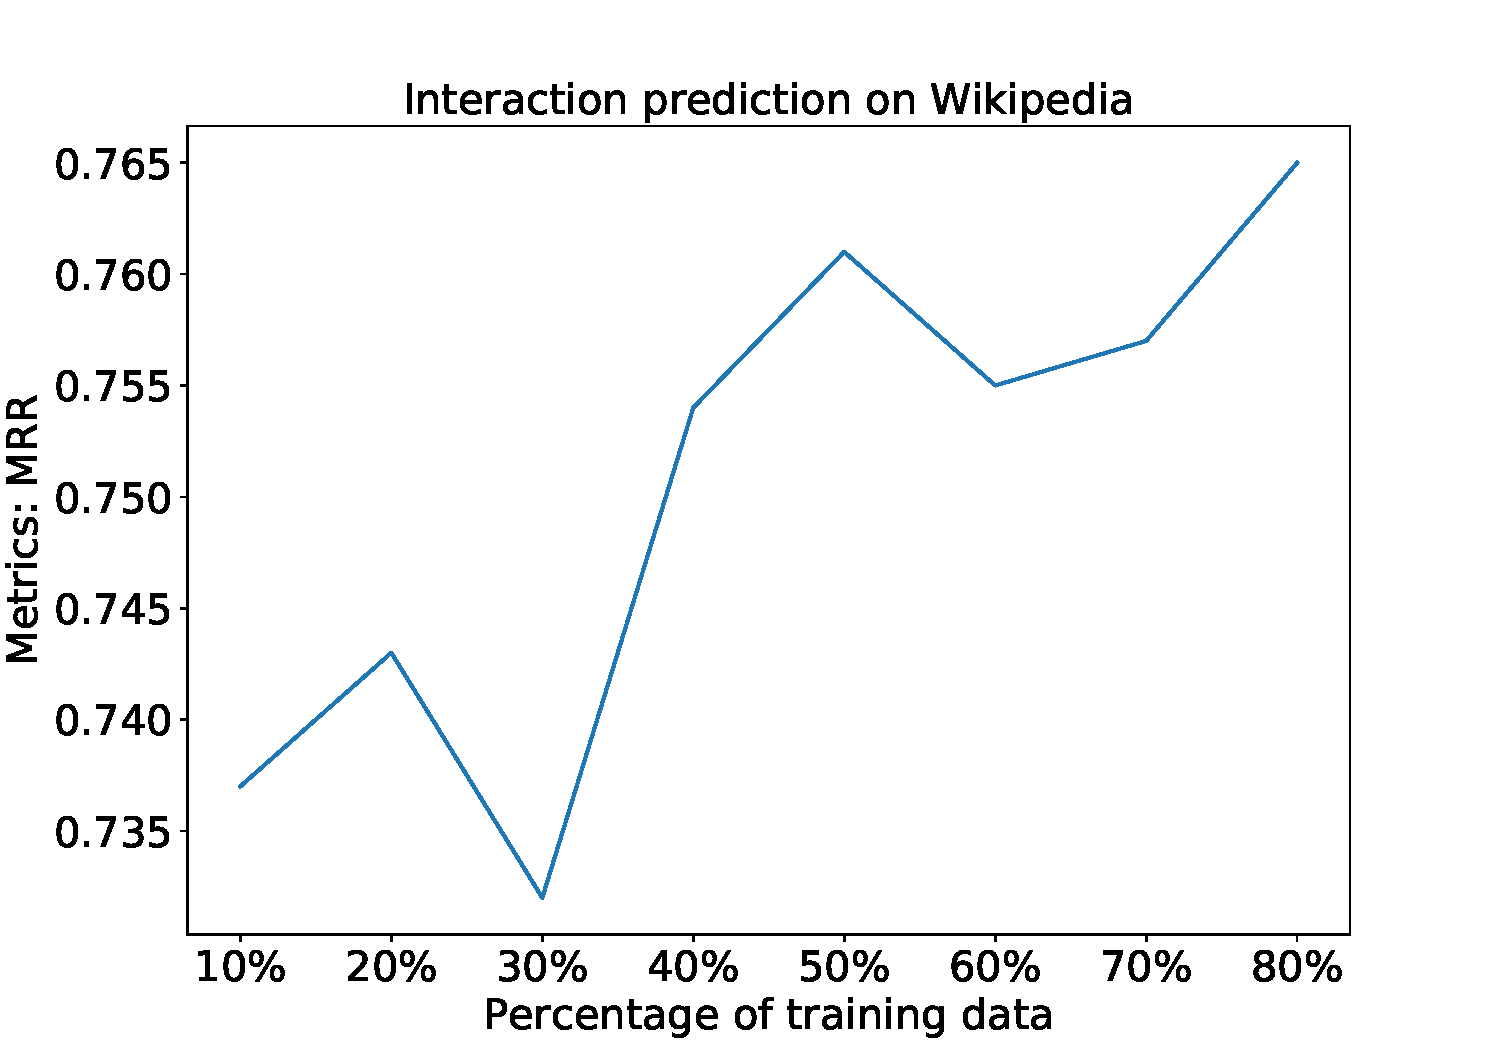
\includegraphics[width=1\textwidth]{image/wiki.pdf}
%    \end{subfigure}
%    \begin{subfigure}[b]{0.49\textwidth}
%        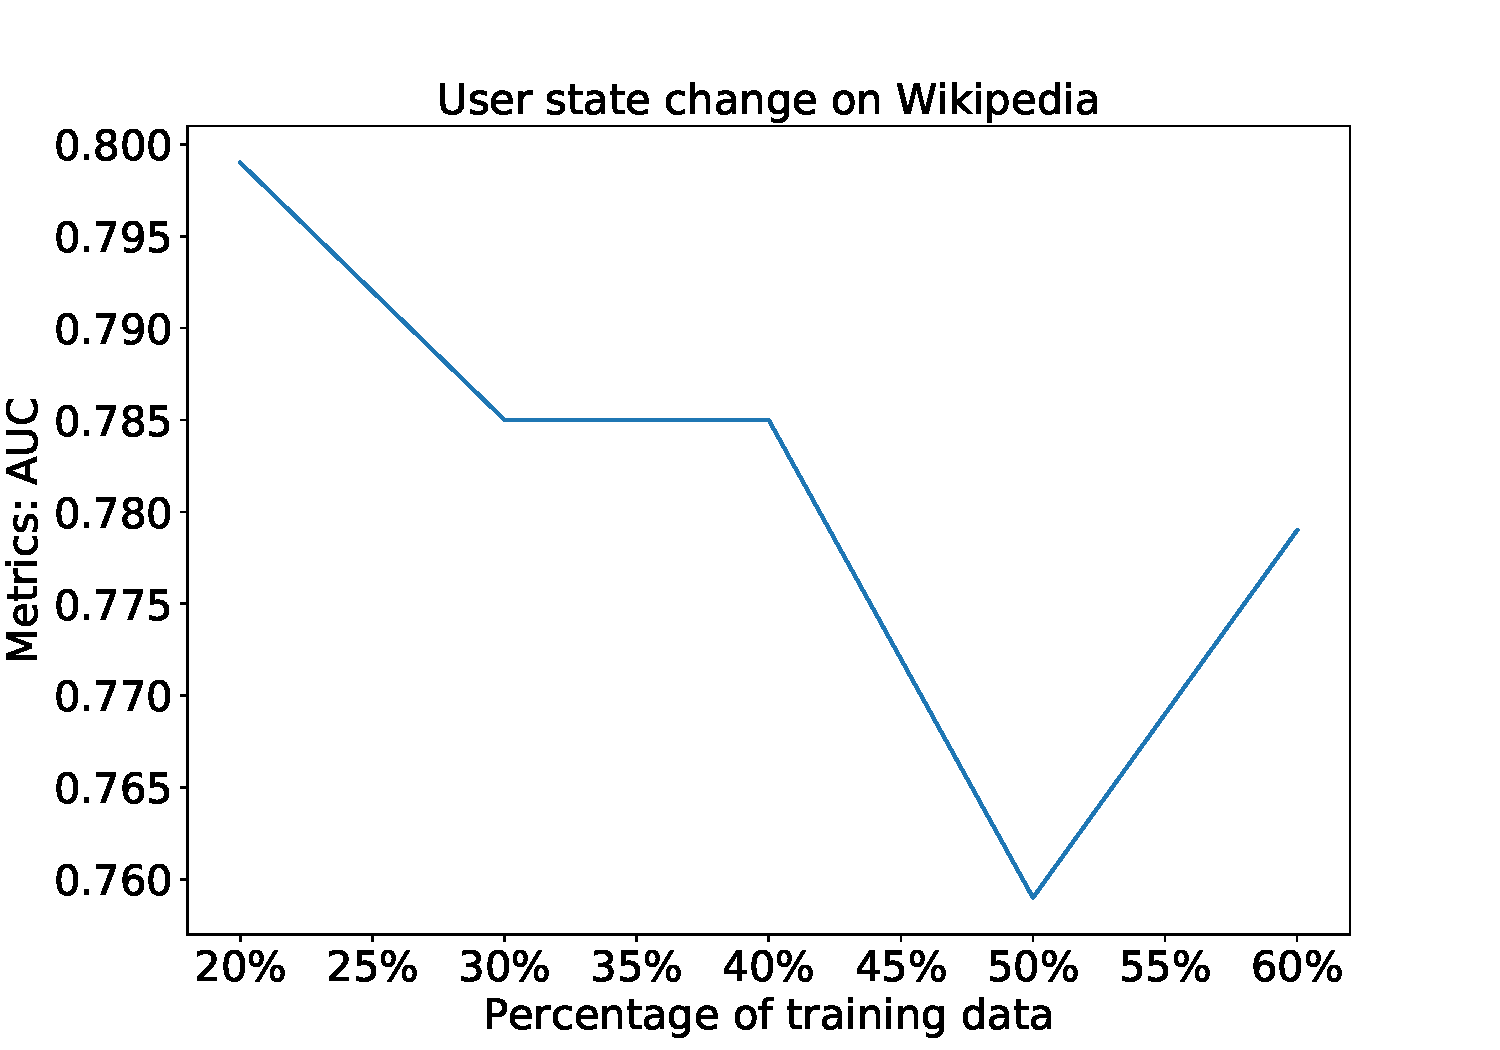
\includegraphics[width=1\textwidth]{image/wiki_state.pdf}
%    \end{subfigure}

%    \caption{Robustness of JODIE replication: [A] compare the MRR of JODIE replication with baselines on interaction prediction task, by varying the training data size. [B] shows the AUC of user state change prediction task by varying the training data size.}
%    \label{fig:foobar}
%\end{figure}

We can see on the first figure that shows an increasing curve. The larger the training set is, the better is the model in the prediction of future interaction. This is because the test set is reduced each time. If we were to compare the curve obtained by the authors of the paper and ours, we could say that the general shape is similar.
For the second figure, the curve is decreasing. The larger the training set is, the more the model is wrong. In state prediction, there is very few change of state so the model will tend to predict more the majority class when the training set is smaller and does not contains enough changing state cases. This is even more pronounced when the training set get even smaller.\\

Additionally, we test the robustness of the model for variations in the size of the embeddings. The figure on the left shows the MRR results of predicting future interactions for the datasets LastFM and Wikipedia and the figure on the right shows the same results but in recall@10:
\begin{figure}[H]
    \centering
    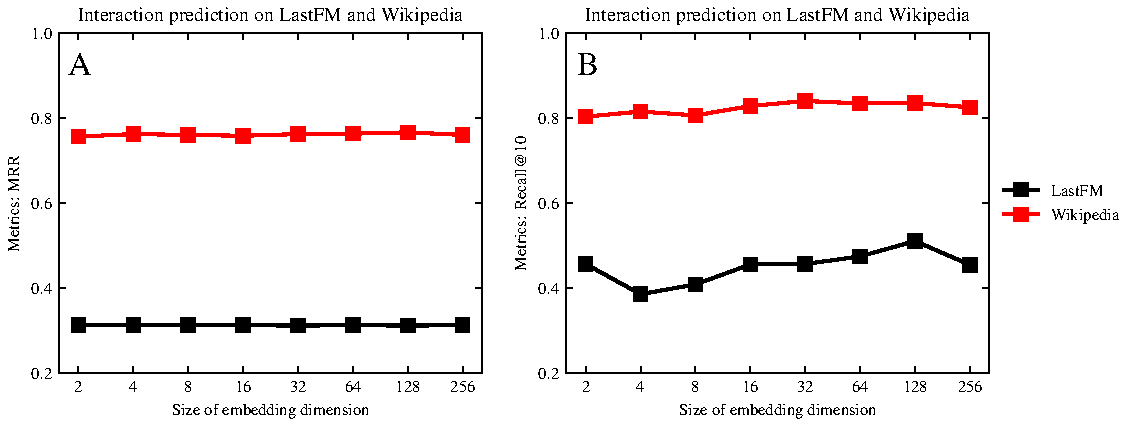
\includegraphics[width = \textwidth]{image/lastFM-wiki.pdf}
    \caption{Robustness of JODIE replication}
\end{figure}
In the original paper, the authors performed this experiment for embedding sizes of 32, 64, 128 and 256 on LastFM. Here , we proposed to do the same experiment but with two additional embedding sizes 8 and 16 but also to add a dataset which is Wikipedia, to test if the claiming of the original paper is generalizable. We see that whatever the size of the embeddings, we obtain stable MRR performances for both datasets. To go further, we decide to draw the same curves but for the recall@10. On this figure, we can see that there is indeed an increase in performance. As we can see the robustness of the model is depending on the metric choice.\\


We can say that their model outperforms the existing models on these 4 datasets and that for these results the replication and reproduction are validated.

\subsection*{Additional result not present in the original paper}

To go further, we decided to test the impact of the \texttt{split} hyper-parameter. As a reminder, the original study does not consider \texttt{split} as a hyper-parameter but as a fixed value of 500. The following figures show the importance of choosing this hyper-parameter. To do so, we predict the user state change on MOOC dataset with several embedding sizes 8, 16 and 32 and different split 5, 500 and 50000.

\begin{figure}[H]
	\centering
    \begin{subfigure}[b]{0.30\textwidth}
        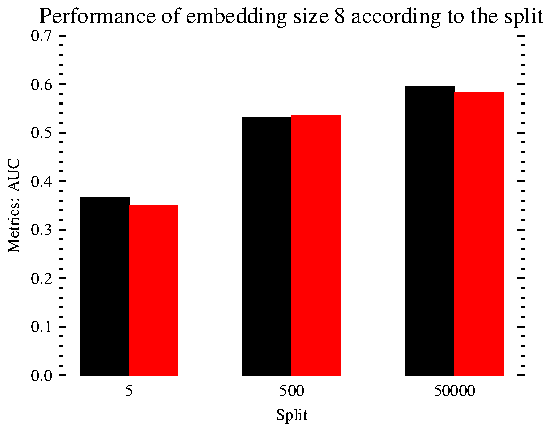
\includegraphics[width=\textwidth]{image/8_split.pdf}
    \end{subfigure}
    \begin{subfigure}[b]{0.30\textwidth}
        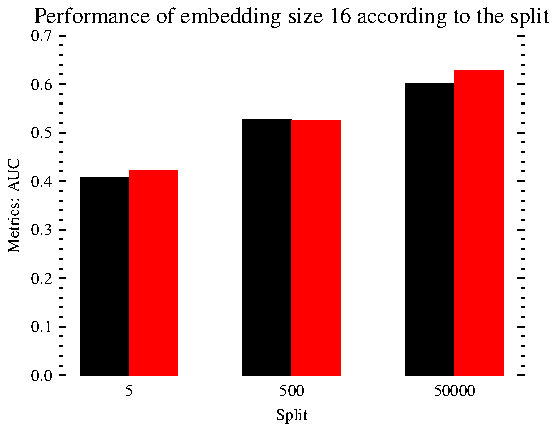
\includegraphics[width=\textwidth]{image/16_split.pdf}
    \end{subfigure}
    \begin{subfigure}[b]{0.36\textwidth}
        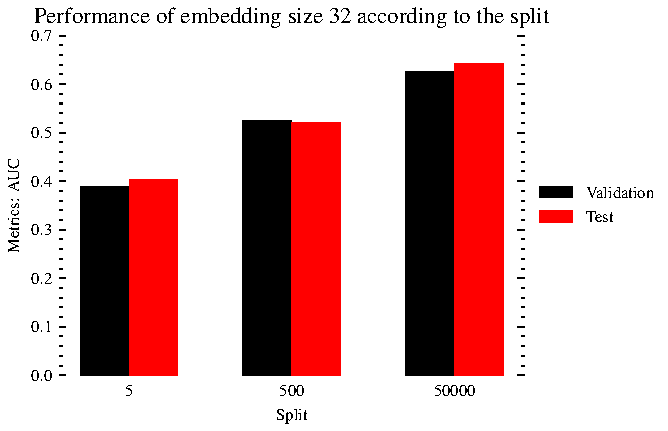
\includegraphics[width=\textwidth]{image/32_split.pdf}
    \end{subfigure}
    \caption{Robustness of JODIE replication: [A] compare the MRR of JODIE replication with baselines on interaction prediction task, by varying the training data size. [B] shows the AUC of user state change prediction task by varying the training data size.}
    \label{fig:foobar}
\end{figure}

We can see, for any embedding size, that the performance is increasing when the \texttt{split} values is high. By increasing this \texttt{split} value from 5 to 500, we have increased the performance by 0.14 in AUC for the different sizes of embedding. Going from 500 to 50000, increased the performance by 0.08. We can say that the choice of this hyper-parameter is important to have better performance. We can explain this improvement by the fact that the model will do back-propagation after each time step defined by \texttt{split}. So if we increase the \texttt{split} number, we increase the number of back-propagation. This suggest that higher values of this parameter allows to enhance the performance but the choice of it must been done considering the running time and the complexity which are increasing significantly when the \texttt{split} get larger.

\section*{Conclusion}
With our work we are able to successfully reproduce the results obtained by the authors of the original paper. As explained in the previous section, some of our results differ slightly from those in the paper. This can be explained by a variation due to the initialization but also by the evaluation of the last epoch for the replication while the authors of the paper evaluated each epoch and chose the best performance on the validation. We can say that the JODIE model outperforms the state of the art methods.\\
Our replication allowed to make a more readable code, easily reusable and easily adjustable for all the hyper-parameters combinations.\\
We also tested the importance of the hyper-parameter \texttt{split}. It was concluded that it is important to choose well to obtain better results. The highest performance was obtained with the largest value but a learning time that is longer. This hyper-parameter must be adjusted taking into account a complexity-performance trade-off.\\
In terms of perspectives, it would be interesting to use the focal loss\supercite{https://doi.org/10.48550/arxiv.1708.02002}. We use this loss in cases of unbalanced class. This loss allowed to have better results in these cases.